\documentclass[11pt,letterpaper,onecolumn]{article}
\usepackage[utf8]{inputenc}
\usepackage[T1]{fontenc}
\usepackage[letterpaper,top=2.54cm,bottom=2.54cm,left=2.54cm,right=2.54cm]{geometry}
\usepackage{mathtools}
\usepackage{amsmath}
\usepackage{amsthm}
\usepackage{newtxtext,newtxmath}
\newtheorem{definition}{Definition}
\newtheorem{remark}{Remark}
\usepackage{booktabs}
\usepackage{array}
\usepackage{multirow}
\usepackage{tabularx}
\usepackage{enumitem}
\usepackage{titlesec}
\usepackage{caption}
\captionsetup{font=small,labelfont=bf,labelsep=period,justification=raggedright,singlelinecheck=false}
\titlespacing*{\section}{0pt}{11pt}{3pt}
\titlespacing*{\subsection}{0pt}{9pt}{2.5pt}
\titlespacing*{\subsubsection}{0pt}{7pt}{2pt}
\titleformat{\section}{\large\bfseries}{\thesection}{0.6em}{}
\titleformat{\subsection}{\normalsize\bfseries\itshape}{\thesubsection}{0.6em}{}
\titleformat{\subsubsection}{\normalsize\itshape}{\thesubsubsection}{0.6em}{}

\usepackage{tikz}
\usepackage{pgfplots}
\pgfplotsset{compat=1.18}
\usetikzlibrary{arrows.meta,positioning,shapes.geometric,fit,calc,plotmarks}
\usepackage{algorithm}
\usepackage{algorithmicx}
\usepackage{algpseudocode}
\algrenewcommand\algorithmicrequire{\textbf{Input:}}
\algrenewcommand\algorithmicensure{\textbf{Output:}}
\usepackage{graphicx}
\usepackage{adjustbox}
\usepackage{xcolor}
\usepackage{cite}
\usepackage{xurl}
\usepackage[colorlinks=true,allcolors=blue!60!black,breaklinks=true]{hyperref}
\usepackage{fancyhdr}

\pagestyle{fancy}
\fancyhf{}
\fancyhead[L]{\footnotesize\textit{Computers, Materials \& Continua}}
\fancyhead[R]{\footnotesize\thepage}
\renewcommand{\headrulewidth}{0.4pt}
\setlength{\parindent}{0.20in}
\setlength{\parskip}{1.8pt}
\renewcommand{\baselinestretch}{1.05}
\emergencystretch=1.5em
\setcounter{topnumber}{2}
\setcounter{bottomnumber}{2}
\setcounter{totalnumber}{3}
\renewcommand{\topfraction}{0.85}
\renewcommand{\bottomfraction}{0.80}
\renewcommand{\textfraction}{0.15}
\renewcommand{\floatpagefraction}{0.75}
\setlength{\textfloatsep}{10pt plus 2pt minus 2pt}
\setlength{\floatsep}{8pt plus 2pt minus 2pt}

\hypersetup{pdftitle={Verified Localized Episodic Grounding with Counterexample Rule Refinement for Auditable LLM-Assisted Network Traffic Analysis}}

\begin{document}

\noindent{\fontsize{14}{18}\selectfont\bfseries Verified Localized Episodic Grounding with Counterexample Rule Refinement for Auditable LLM-Assisted Network Traffic Analysis\par}
\vspace{0.55em}

\noindent{\fontsize{10}{13}\selectfont\bfseries Ye Tang$^{1,\#}$, Ruikai Han$^{1,\#}$, Yi Hu$^{1,*}$ and Ruzhen Chen$^{2,*}$}\\[0.35em]
{\fontsize{10}{12.5}\selectfont
\noindent$^{1}$School of Information Science and Technology, Xizang University, Lhasa, 850000, China\\
$^{2}$School of Education, Xizang University, Lhasa, 850000, China\\
$^{*}$Corresponding Authors: Yi Hu. Email: hy610400@163.com; Ruzhen Chen. Email: crz@xzu.edu.cn\\
$^{\#}$These authors contributed equally to this work\\
Received: XX Month 2026; Accepted: XX Month 2026
\par}

\vspace{0.55em}
\hrule
\vspace{0.45em}
{\fontsize{10}{12.5}\selectfont
\noindent\textbf{Abstract:} Memory-augmented large language models (LLMs) can support few-shot network intrusion triage by distilling historical flows into human-auditable rules without gradient updates, yet local reflections suffer from label hallucination, cross-flow over-generalization, and prompt anchoring on non-firing rules. We propose Verified Localized Episodic Grounding (VLEG) and its counterexample-refined neuro-symbolic extension (VLEG-CR-NS) for auditable few-shot network traffic analysis. During offline consolidation, VLEG verifies candidate reflections against their labeled source records within $K$ attempts, after which a deterministic compiler parses admitted heuristics into executable Boolean predicates and feeds within-seed contrary-label counterexamples back to the generator to specialize overly broad rules. On a 16-scene symbolic benchmark, source verification ($K=3$) eliminates label inversions ($100\%$ source agreement) and matches raw retrieval accuracy at 70B ($91.67\%$ versus $89.58\%$). On deduplicated 19-feature UNSW-NB15 telemetry across five 32-flow seeds and 1,000 shared test fingerprints, unverified reflection mislabels $95.0\%$ ($76/80$) of malicious support flows as benign ($42.66\%$ Macro-F1). Stage-A VLEG restores $100\%$ source-label agreement across $158/160$ admitted episodes ($59.68\%$ Macro-F1), but $59.2\%$ ($93/157$) of parseable rules match within-seed counterexamples. Stage-B counterexample refinement (VLEG-CR) raises total zero-counterexample rule coverage from $40.0\%$ ($64/160$) to $83.1\%$ ($133/160$, or $84.2\%$ of the $158$ Stage-A admitted episodes) and cuts unseen cross-seed counterexamples from $72.0\%$ to $40.6\%$. Executing compiled zero-counterexample predicates deterministically before falling back to raw retrieval avoids LLM false alarms induced by non-firing prompt text: VLEG-CR-NS reaches $64.88\%$ Macro-F1 ($+0.96$ percentage points over raw retrieval, $95\%$ confidence interval $[+0.19, +1.71]$), while Pilot-selected bank triage (VLEG-CR-Bank, $\tau_{\mathrm{sup}}=3$) achieves $65.30\%$ Macro-F1 ($+1.38$ percentage points, $95\%$ confidence interval $[+0.18, +2.61]$) and reduces the false positive rate to $35.99\%$ (lowest across all LLM, neuro-symbolic, unconstrained-tree, and ensemble baselines) while saving $47.1\%$--$49.0\%$ of online LLM calls. Delegating uncovered boundary flows to a 32-flow shallow decision tree without hyperparameter re-tuning further lifts Macro-F1 to $67.05\%$--$67.57\%$ at zero online LLM cost.\par
\vspace{0.35em}
\noindent\textbf{Keywords:} Episodic memory; hallucination mitigation; large language models; network traffic analysis; intrusion detection; counterexample-guided refinement; neuro-symbolic execution
\par}
\vspace{0.45em}
\hrule
\vspace{0.55em}

\section{Introduction}
\subsection{Background and Motivation}
Large language models (LLMs) can utilize retrieved demonstrations in the prompt to classify structured telemetry and assist security incident response without parameter updates \cite{brown2020language,lewis2020retrieval}. In enterprise network traffic analysis and Security Operations Center (SOC) alert triage \cite{lin2022etbert,sharafaldin2018cicids,papamartzivanos2018dendron,jacobs2022ai}, analysts routinely examine emerging attack patterns under severe label scarcity, where only a few dozen vetted historical flows are available. Classical tabular learners such as Classification and Regression Trees (CART), Random Forest (RF), and Gradient Boosting Decision Trees (GBDT) offer fast inference and strong discriminative recall, yet univariate axis-aligned splits lack protocol-level semantics and cross-feature relational expressions \cite{wei2023xaiids,charmet2022explainable}. Conversely, feeding historical telemetry to an LLM promises readable triage rationales \cite{houssel2024explainable,islam2026maids,guastalla2024llmdos}, but finite and unevenly attended context windows make performance highly sensitive to how historical evidence is consolidated and presented \cite{an2025why,liu2024lost}.

Persistent-memory architectures extend agent experience beyond fixed prompts by storing episodic records or distilled textual abstractions \cite{packer2023memgpt,wang2023longmem,wang2024memoryllm,gutierrez2024hipporag,maharana2024evaluating}. Retaining raw flow records preserves instance-level fidelity, whereas summarizing flows into explicit \texttt{if-then} heuristics provides reusable decision guidance. However, unconstrained natural-language reflection introduces three cascading reliability hazards. First, an unverified reflection can invert a flow's true class label or hallucinate unrecorded packet fields. Second, a reflection that agrees with its single originating flow can still over-generalize across broader traffic by latching onto common transport states shared with benign connections. Third, even when a rule is specialized to exclude contrary-label counterexamples, displaying its text inside an LLM prompt on target flows where its antecedent evaluates to false can still bias a quantized LLM toward false alarms via textual label anchoring.

Consequently, single-episode source fidelity, cross-episode rule specificity, and inference-time execution fidelity constitute distinct design dimensions that cannot be solved by single-pass prompting alone. Auditing and closing this loop requires coupling per-episode verification with deterministic cross-flow counterexample refinement and symbolic rule execution.

\subsection{Research Scope and Study Positioning}
Recent agentic memory systems combine episodic retrieval with verbal reflection or global hypothesis induction \cite{wu2025from,zhang2025survey,shinn2023reflexion,wang2024voyager,agarwal2026hypothesis,he2024idea}. Our work investigates how localized episodic reflections behave under strict source verification and cross-episode counterexample constraints when applied to deduplicated network flow telemetry. Specifically, we examine whether iterative source verification eliminates label-inversion collapse without suppressing incidental distractors, why source-verified heuristics still trigger false alarms across unseen support banks, and how deterministic predicate compilation can both refine over-generalized rules offline and replace error-prone prompt interpretation online. Rather than treating LLM memory in isolation, we situate neuro-symbolic rule triage directly alongside raw-feature retrieval, shallow CART decision trees, and ensemble classifiers under identical support-set budgets.

\subsection{Proposed Two-Phase VLEG-CR and Neuro-Symbolic Triage Framework}
We propose Verified Localized Episodic Grounding (VLEG), extended with Counterexample-Refined consolidation (VLEG-CR) and Neuro-Symbolic rule triage (VLEG-CR-NS and VLEG-CR-Bank). During offline Phase~1 consolidation, a generator proposes a testable local heuristic from flow features, and an independent verifier checks label agreement and attribute faithfulness against the source episode within $K$ attempts (Stage~A). Admitted Stage-A heuristics are then parsed by a deterministic compiler $\Psi$ into executable Boolean predicates over the 19 flow features and tested against the remaining 31 support flows in the same seed bank (Stage~B). Rules matching contrary-label counterexamples receive structured counterexample critiques and separating feature bounds for up to $K_{\mathrm{CR}}$ inductive refinement steps, committing only rules that pass both $\mathrm{CE}_{\mathrm{seed}}=0$ compilation and source verification while prohibiting exact-equality memorization on continuous features.

During online Phase~2 inference, VLEG-CR-NS and VLEG-CR-Bank evaluate compiled zero-counterexample predicates deterministically on the target flow in sub-millisecond CPU time. Queries matched unambiguously by firing rules return deterministic predictions and human-readable protocol rationales immediately at zero LLM cost; uncovered or conflicting boundary queries fall back either to top-$k$ raw-flow LLM inference or to a lightweight shallow CART tree fitted on the same 32 support flows.

\subsection{Summary of Contributions}
Evaluated across a multi-level symbolic benchmark at 7B and 70B scales and a five-seed benchmark over deduplicated UNSW-NB15 network flows \cite{moustafa2015unsw}, this study makes four contributions:
\begin{itemize}[leftmargin=1.8em,topsep=2pt,itemsep=2pt]
    \item \textbf{Two-Stage Verified and Counterexample-Refined Consolidation:} We design a closed-loop consolidation pipeline uniting LLM source verification with a deterministic predicate compiler $\Psi$ that iteratively eliminates within-bank counterexamples while blocking float-literal memorization.
    \item \textbf{Mechanistic Isolation of Three Reflection Failure Modes:} Across synthetic scenes and real network flows, we disentangle unverified malicious-to-benign label collapse (including under a label-informed unverified control), cross-flow over-generalization of source-consistent rules, and LLM false-positive anchoring induced by non-firing rules in hybrid prompts.
    \item \textbf{Neuro-Symbolic Triage Surpassing Raw Retrieval with Lower Compute:} Coupling counterexample-refined rules with deterministic symbolic execution yields statistically significant Macro-F1 gains of up to $+1.38$ percentage points over raw flow retrieval, reduces false positives below raw retrieval and all 32-flow unconstrained-tree and ensemble baselines, and eliminates nearly half of online 70B LLM calls.
    \item \textbf{Complementary Integration with Shallow Decision Trees:} Benchmarking against leak-free 32-flow CART, RF, and GBDT models clarifies the trade-off between global impurity optimization and modular relational rules, demonstrating that routing uncovered boundary flows to a shallow CART fallback eliminates $100\%$ of online LLM calls (and $100\%$ of online embedding calls in Bank scope) while matching or surpassing 32-flow GBDT in Macro-F1 with lower false-alarm rates.
\end{itemize}

\subsection{Paper Organization}
Section~2 reviews retrieval-augmented memory, iterative rule induction, and explainable network intrusion detection. Section~3 formalizes VLEG, the VLEG-CR compiler and refinement loop, the 19-feature representation, and neuro-symbolic triage. Section~4 presents the symbolic sanity check, the UNSW-NB15 benchmark, factorial ablations, cost audits, and CART integration, followed by limitations. Section~5 concludes the study.

\section{Related Work}
\subsection{Episodic Retrieval and Persistent LLM Memory}
Retrieval-augmented architectures ground LLM predictions in external demonstrations without weight updates \cite{brown2020language,lewis2020retrieval}, where demonstration selection strongly governs in-context accuracy \cite{zhang2022active,purohit2025sample}. Long-horizon agent frameworks manage finite context budgets \cite{an2025why,liu2024lost} through hierarchical paging in MemGPT \cite{packer2023memgpt}, decoupled memory encoders in LongMem \cite{wang2023longmem} and MemoryLLM \cite{wang2024memoryllm}, personalized forgetting curves in MemoryBank \cite{zhong2024memorybank}, and associative indexing in HippoRAG \cite{gutierrez2024hipporag}. Longitudinal evaluations such as LoCoMo \cite{maharana2024evaluating} and recent memory surveys \cite{wu2025from,zhang2025survey} show that uncurated episodic logs accumulate noise, whereas Generative Agents \cite{park2023generative}, A-MEM \cite{xu2025amem}, and timeline-based dialogue managers \cite{kim2024towards} compress episodes into textual reflections without formal cross-episode false-positive verification.

\subsection{Self-Refinement, Verification, and Inductive Rule Learning}
Iterative feedback loops improve LLM reliability through verbal trial-and-error in Reflexion \cite{shinn2023reflexion}, executable skill verification in Voyager \cite{wang2024voyager}, intrinsic critique in Self-Refine \cite{madaan2023selfrefine}, consistency sampling in SelfCheckGPT \cite{manakul2023selfcheckgpt}, factored verification in Chain-of-Verification \cite{dhuliawala2024chain}, and external tool feedback in CRITIC \cite{gou2024critic}. For explicit rule learning, Hypothesis-Driven Reasoning (HDR) \cite{agarwal2026hypothesis} and IDEA \cite{he2024idea} consolidate observations into global rule sets, while recent inductive benchmarks examine abstraction playgrounds \cite{kim2022playgrounds}, hypothesis refinement \cite{qiu2024phenomenal}, diverse hypothesis generation \cite{lee2025generating}, and open-ended scientific discovery \cite{zhou2024hypothesis}. Complementary multi-store cognitive architectures coordinate episodic and semantic tiers \cite{kim2023machine,li2024memory,wang2025mirix}. Unlike global rule compression, which degrades under conditional exceptions, VLEG-CR maintains localized episode provenance while using deterministic counterexample compilation to enforce bank-wide consistency.

\subsection{Explainable Network Traffic Analysis and Intrusion Detection}
Machine learning for encrypted and tabular traffic classification spans pre-trained datagram transformers such as ET-BERT \cite{lin2022etbert}, benchmark flow corpora including UNSW-NB15 \cite{moustafa2015unsw} and CICIDS2017 \cite{sharafaldin2018cicids}, and operational deployment frameworks such as Kitsune \cite{mirsky2018kitsune} and pitfalls-aware evaluation protocols \cite{arp2022dos}. Because black-box classifiers hinder incident response, explainable intrusion detection research has explored evolutionary decision rules in Dendron \cite{papamartzivanos2018dendron}, trustee-extracted symbolic trees \cite{jacobs2022ai}, post-hoc attribution frameworks \cite{wei2023xaiids,charmet2022explainable}, and deep anomaly detectors in network security venues \cite{alissa2022botnet}. More recently, LLM-assisted IDS prototypes have investigated zero-shot flow explanation \cite{houssel2024explainable}, multi-agent RAG experience libraries in MA-IDS \cite{islam2026maids}, and DDoS packet prompting \cite{guastalla2024llmdos}. Our study advances this line by diagnosing why prompt-injected LLM reflections hallucinate and over-generalize on deduplicated flows, and by uniting compiled LLM relational predicates with raw retrieval and shallow CART trees.

\section{The Proposed Method}
\subsection{Problem Formulation and Architecture Overview}
Consider a small labeled historical support bank $\mathcal{E}_{\mathrm{seed}} = \{e_1, e_2, \dots, e_N\}$, where each episode $e_i = (x_i, y_i)$ pairs a structured feature vector $x_i \in \mathcal{X}$ with a ground-truth class label $y_i \in \mathcal{Y}$. Given an unlabeled target query $T = (x_T)$, the system must predict $\hat{y}_T \in \mathcal{Y}$ while providing human-auditable evidence grounded in $\mathcal{E}_{\mathrm{seed}}$ without updating LLM parameters.

\begin{figure}[tbp]
\centering
\begin{adjustbox}{max width=0.98\textwidth}
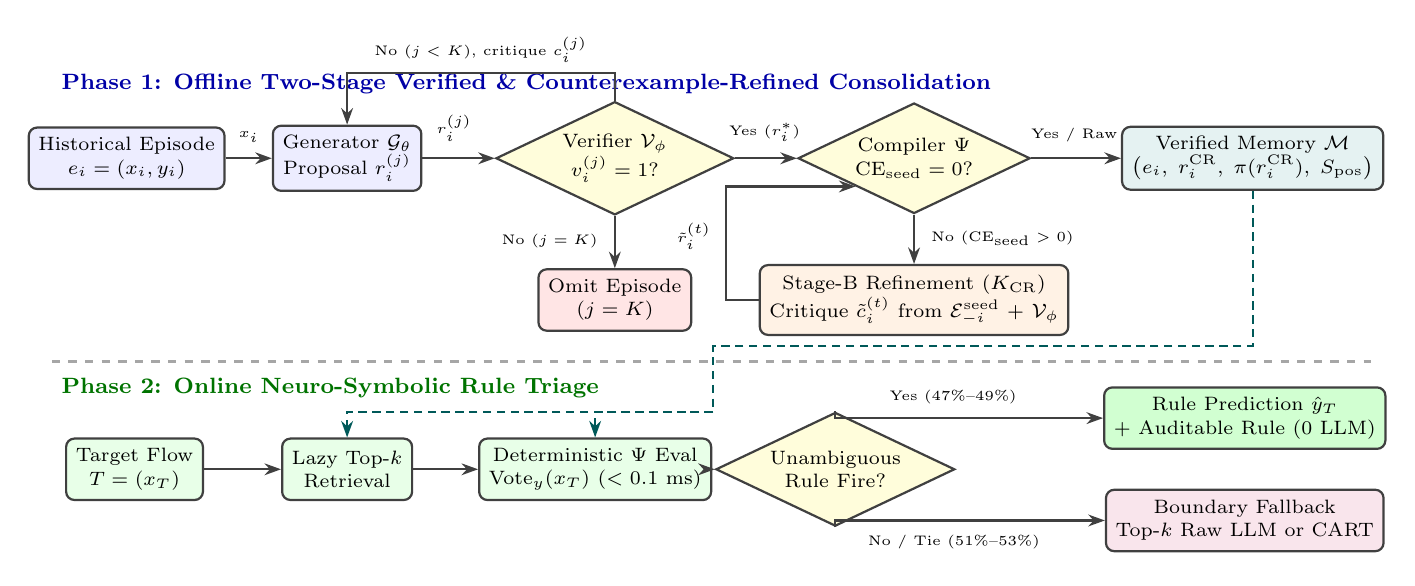
\begin{tikzpicture}[
    font=\scriptsize,
    box/.style={rectangle, rounded corners=3pt, draw=black!75, thick, align=center, minimum height=0.78cm, inner sep=3.5pt},
    stageA/.style={box, fill=blue!7},
    stageB/.style={box, fill=orange!10},
    mem/.style={box, fill=teal!10, minimum width=2.85cm},
    phase2/.style={box, fill=green!9},
    dec/.style={diamond, aspect=2.1, draw=black!75, thick, fill=yellow!14, align=center, inner sep=1.8pt},
    arr/.style={-{Stealth[length=2.1mm,width=1.5mm]}, thick, draw=black!75}
]
% Phase 1 Banner
\node[anchor=west, font=\footnotesize\bfseries, text=blue!65!black] at (-0.1, 2.95) {Phase 1: Offline Two-Stage Verified \& Counterexample-Refined Consolidation};
\node[stageA] (ep) at (0.85, 2.00) {Historical Episode\\$e_i = (x_i, y_i)$};
\node[stageA] (genA) at (3.65, 2.00) {Generator $\mathcal{G}_\theta$\\Proposal $r_i^{(j)}$};
\node[dec] (verA) at (7.05, 2.00) {Verifier $\mathcal{V}_\phi$\\$v_i^{(j)} = 1$?};
\node[box, fill=red!10] (drop) at (7.05, 0.20) {Omit Episode\\($j = K$)};

\node[dec] (comp) at (10.85, 2.00) {Compiler $\Psi$\\$\mathrm{CE}_{\mathrm{seed}}=0$?};
\node[stageB] (genB) at (10.85, 0.20) {Stage-B Refinement ($K_{\mathrm{CR}}$)\\Critique $\tilde{c}_i^{(t)}$ from $\mathcal{E}_{-i}^{\mathrm{seed}}$ + $\mathcal{V}_\phi$};
\node[mem] (bank) at (15.15, 2.00) {Verified Memory $\mathcal{M}$\\$\big(e_i,\; r_i^{\mathrm{CR}},\; \pi(r_i^{\mathrm{CR}}),\; S_{\mathrm{pos}}\big)$};

\draw[arr] (ep) -- node[above=2pt, font=\tiny]{$x_i$} (genA);
\draw[arr] (genA) -- node[above=2.5pt, pos=0.44, font=\tiny]{$r_i^{(j)}$} (verA);
\draw[arr] (verA.north) -- ++(0,0.35) -| node[pos=0.25, above, font=\tiny]{No ($j < K$), critique $c_i^{(j)}$} (genA.north);
\draw[arr] (verA.south) -- node[left=2.5pt, pos=0.48, font=\tiny]{No ($j = K$)} (drop.north);
\draw[arr] (verA) -- node[above=2.2pt, pos=0.48, font=\tiny]{Yes ($r_i^*$)} (comp);
\draw[arr] (comp.south) -- node[right=2.5pt, pos=0.48, font=\tiny]{No ($\mathrm{CE}_{\mathrm{seed}}>0$)} (genB.north);
\draw[arr] (genB.west) -- ++(-0.42,0) |- node[pos=0.28, left=1.5pt, font=\tiny]{$\tilde{r}_i^{(t)}$} (comp.south west);
\draw[arr] (comp) -- node[above=2.2pt, pos=0.48, font=\tiny]{Yes / Raw} (bank);

% Divider
\draw[dashed, gray!70, thick] (-0.1, -0.58) -- (16.65, -0.58);

% Phase 2 Banner
\node[anchor=west, font=\footnotesize\bfseries, text=green!45!black] at (-0.1, -0.92) {Phase 2: Online Neuro-Symbolic Rule Triage};
\node[phase2] (query) at (0.95, -1.95) {Target Flow\\$T = (x_T)$};
\node[phase2] (ret) at (3.65, -1.95) {Lazy Top-$k$\\Retrieval};
\node[phase2] (exec) at (6.80, -1.95) {Deterministic $\Psi$ Eval\\$\mathrm{Vote}_y(x_T)$ ($< 0.1$~ms)};
\node[dec] (fire) at (9.85, -1.95) {Unambiguous\\Rule Fire?};
\node[box, fill=green!18, minimum width=3.15cm] (out1) at (15.05, -1.30) {Rule Prediction $\hat{y}_T$\\+ Auditable Rule (0 LLM)};
\node[box, fill=purple!10, minimum width=3.15cm] (out2) at (15.05, -2.60) {Boundary Fallback\\Top-$k$ Raw LLM or CART};

\draw[arr] (query) -- (ret);
\draw[arr, densely dashed, teal!70!black] (bank.south) -- (15.15, -0.38) -- (8.30, -0.38) -- (8.30, -1.22) -| (ret.north);
\draw[arr, densely dashed, teal!70!black] (8.30, -1.22) -| (exec.north);
\draw[arr] (ret) -- (exec);
\draw[arr] (exec) -- (fire);
\draw[arr] (fire.north) |- node[pos=0.72, above=1.5pt, font=\tiny]{Yes ($47\%$--$49\%$)} (out1.west);
\draw[arr] (fire.south) |- node[pos=0.72, below=1.5pt, font=\tiny]{No / Tie ($51\%$--$53\%$)} (out2.west);
\end{tikzpicture}
\end{adjustbox}
\caption{Two-phase architecture of VLEG-CR and Neuro-Symbolic Rule Triage. Phase~1 combines Stage-A per-episode verification ($K$) with Stage-B deterministic counterexample refinement ($K_{\mathrm{CR}}$). Phase~2 evaluates verified $\mathrm{CE}_{\mathrm{seed}}=0$ predicates deterministically within $0.1$~ms before routing uncovered boundary queries to raw-retrieval LLM inference or a shallow CART tree.}
\label{fig:architecture}
\end{figure}

Figure~\ref{fig:architecture} illustrates the complete two-phase workflow. Rather than compressing $\mathcal{E}_{\mathrm{seed}}$ into a single brittle global prompt or committing unverified per-flow reflections, our framework enforces three sequential safeguards: (1) Stage-A source verification eliminates label inversions and fabricated attributes on each originating episode $e_i$; (2) Stage-B counterexample-guided refinement specializes rules via compiler $\Psi$ until within-seed contrary-label matches reach zero; and (3) Phase-2 neuro-symbolic triage executes compiled predicates deterministically on $x_T$ so that non-firing rules never pollute an LLM inference prompt.

\subsection{Stage-A Bounded Per-Episode Source Verification (VLEG)}
For each support episode $e_i = (x_i, y_i)$ and iteration index $j \in \{0, 1, \dots, K-1\}$, generator $\mathcal{G}_\theta$ proposes a localized heuristic $r_i^{(j)}$ according to Eq.~(\ref{eq:stage_a_gen}):
\begin{equation}
\label{eq:stage_a_gen}
    r_i^{(j)} \sim \begin{cases}
        \mathcal{G}_\theta(\cdot \mid x_i), & \text{if } j = 0, \\[3pt]
        \mathcal{G}_\theta\big(\cdot \mid x_i,\; r_i^{(j-1)},\; c_i^{(j-1)}\big), & \text{if } 1 \le j \le K-1.
    \end{cases}
\end{equation}
At the initial proposal $j = 0$, $\mathcal{G}_\theta$ observes only the feature representation $x_i$ without $y_i$. Withholding $y_i$ at $j = 0$ prevents trivial label parroting (e.g., outputting ``\texttt{if proto == tcp then MALICIOUS}'' merely to echo a given label) and tests whether the generator's zero-shot prior aligns with actual traffic anomalies; as we verify empirically in Section~\ref{sec:exp6}, even providing $y_i$ directly in an unverified single-step prompt still yields $87.3\%$ over-generalized rules without iterative verification.

An independent zero-temperature verifier $\mathcal{V}_\phi$ evaluates $r_i^{(j)}$ against the full labeled episode $e_i = (x_i, y_i)$, returning a strict native-Boolean JSON tuple:
\begin{equation}
\label{eq:stage_a_ver}
    \big(v_i^{(j)},\; c_i^{(j)}\big) = \mathcal{V}_\phi\big(e_i,\; r_i^{(j)}\big), \qquad v_i^{(j)} \in \{0, 1\},
\end{equation}
where $v_i^{(j)} = 1$ holds if and only if $r_i^{(j)}$ states a consequent matching $y_i$, cites only supplied feature values in $x_i$, and provides a checkable condition. Malformed JSON or stringified Booleans evaluate to $v_i^{(j)} = 0$. Let $j_i^* = \min\{j \in \{0, \dots, K-1\} : v_i^{(j)} = 1\}$ denote the first passing index. The Stage-A admission operator $\Gamma_{\mathrm{ver}}$ is:
\begin{equation}
\label{eq:stage_a_gate}
    r_i^* = \Gamma_{\mathrm{ver}}(e_i) = \begin{cases}
        r_i^{(j_i^*)}, & \text{if } \max_{0 \le j \le K-1} v_i^{(j)} = 1, \\[4pt]
        \emptyset, & \text{if } \max_{0 \le j \le K-1} v_i^{(j)} = 0 \;\; \text{(omitted from } \mathcal{M}\text{)}.
    \end{cases}
\end{equation}

\begin{remark}[Scope of Single-Episode Source Verification]
Let $E_j^{\mathrm{src}}$ denote the event that $r_i^{(j)}$ contradicts $y_i$ or fabricates attributes of $x_i$, and let $E_j^{\mathrm{cross}}$ denote the event that $r_i^{(j)}$ falsely matches contrary-label episodes $e_m \in \mathcal{E}_{\mathrm{seed}} \setminus \{e_i\}$. Because $\mathcal{V}_\phi$ inspects only $(x_i, y_i)$ across $j \in \{0, \dots, K-1\}$, Stage~A suppresses $E_j^{\mathrm{src}}$ (modulo verifier false positives) and recovers coverage lost under $K=1$, but has zero observability over $E_j^{\mathrm{cross}}$. Suppressing $E_j^{\mathrm{cross}}$ requires cross-episode counterexample checking in Stage~B.
\end{remark}

\subsection{Stage-B Deterministic Predicate Compiler and Counterexample Refinement (VLEG-CR)}
\label{sec:counterexample_gate}
To eliminate $E_j^{\mathrm{cross}}$ among Stage-A admitted episodes ($r_i^* \neq \emptyset$), we introduce a deterministic rule compiler $\Psi$ and counterexample-guided inductive refinement (\textbf{VLEG-CR}). Candidate traffic heuristics follow the conjunctive grammar \texttt{if <cond\_1> and <cond\_2> ... then label = <CLASS>}. Compiler $\Psi$ parses each clause into an executable relational predicate over the feature dictionary:
\begin{equation}
\label{eq:compiler_pred}
    \pi(r)(x) = \bigwedge_{m=1}^{d} \mathrm{op}_m\big(x[\mathrm{field}_m],\; \mathrm{rhs}_m\big) \in \{0, 1\}, \qquad \hat{y}(r) \in \{\texttt{BENIGN}, \texttt{MALICIOUS}\},
\end{equation}
where $\mathrm{op}_m \in \{=, \neq, >, <, \ge, \le\}$ and $\mathrm{rhs}_m$ is either a numeric/string literal or a second feature reference (enabling relational comparisons such as \texttt{sbytes > dbytes}). To block trivial instance memorization, $\Psi$ rejects exact equality ($=$) against non-zero literals on continuous duration, rate, load, inter-packet, jitter, and byte-count fields, requiring inequality bounds instead.

\begin{definition}[Within-Seed Counterexamples, Positive Support, and Inductive Refinement]
For a Stage-A admitted episode $e_i=(x_i,y_i) \in \mathcal{E}_{\mathrm{seed}}$ and parseable candidate rule $r$, let $\mathcal{E}_{-i}^{\mathrm{seed}} = \mathcal{E}_{\mathrm{seed}} \setminus \{e_i\}$ denote the remaining $N-1$ support flows in the same seed bank. Its within-seed counterexample count $\mathrm{CE}_{\mathrm{seed}}(r)$ and same-class positive support $S_{\mathrm{pos}}(r)$ are:
\begin{equation}
\label{eq:ce_count}
    \mathrm{CE}_{\mathrm{seed}}(r) = \sum_{e_m \in \mathcal{E}_{-i}^{\mathrm{seed}}} \mathbb{I}\!\left(\pi(r)(x_m) = 1 \wedge y_m \neq y_i\right), \quad
    S_{\mathrm{pos}}(r) = \sum_{e_m \in \mathcal{E}_{-i}^{\mathrm{seed}}} \mathbb{I}\!\left(\pi(r)(x_m) = 1 \wedge y_m = y_i\right),
\end{equation}
with $S_{\mathrm{pos}}(\emptyset) = 0$ by convention. An offline diagnostic $\mathrm{CE}_{\mathrm{pool}}(r)$ is defined analogously across all $5N - 1$ other support flows pooled across the five seeds ($\mathcal{E}_{\mathrm{all}} \setminus \{e_i\}$) strictly for post-hoc generalization auditing; $\mathrm{CE}_{\mathrm{pool}}$ is never accessed during consolidation or inference.

If $r_i^*$ fails compilation or exhibits $\mathrm{CE}_{\mathrm{seed}}(r_i^*) > 0$, Stage~B executes up to $K_{\mathrm{CR}}$ refinement steps ($t \in \{0, \dots, K_{\mathrm{CR}}-1\}$, initialized at $\tilde{r}_i^{(-1)} = r_i^*$). At step $t$, $\Psi$ extracts up to three falsely matched contrary-label flows $\mathcal{C}_i^{(t)} \subseteq \mathcal{E}_{-i}^{\mathrm{seed}}$ and univariate separating bounds between $x_i$ and $\mathcal{C}_i^{(t)}$ to form a structured counterexample critique $\tilde{c}_i^{(t)}$, prompting $\mathcal{G}_\theta$:
\begin{equation}
\label{eq:cr_gen}
    \tilde{r}_i^{(t)} \sim \mathcal{G}_\theta\big(\cdot \mid x_i,\; \tilde{r}_i^{(t-1)},\; \tilde{c}_i^{(t-1)}\big).
\end{equation}
Candidate $\tilde{r}_i^{(t)}$ is accepted as $r_i^{\mathrm{CR}}$ at the first step $t$ satisfying valid non-memorizing syntax, source truth $\pi(\tilde{r}_i^{(t)})(x_i)=1$, zero within-seed counterexamples $\mathrm{CE}_{\mathrm{seed}}(\tilde{r}_i^{(t)})=0$, and LLM source verification $\mathcal{V}_\phi(e_i, \tilde{r}_i^{(t)})_v = 1$. If all $K_{\mathrm{CR}}$ attempts fail, the admitted episode retains its raw flow $e_i$ with $r_i^{\mathrm{CR}} = \emptyset$.
\end{definition}

\subsection{Feature Representation, Deduplication, and Dense Retrieval}
\label{sec:features_retrieval}
Raw UNSW-NB15 records contain 42 attributes, including sliding 100-connection window aggregates (\texttt{ct\_srv\_src}, \texttt{ct\_state\_ttl}, \texttt{ct\_dst\_ltm}, etc.), TCP base sequence numbers (\texttt{stcpb}, \texttt{dtcpb}), and session-specific flags (\texttt{is\_sm\_ips\_ports}) that leak temporal burst context across adjacent rows in benchmark splits \cite{arp2022dos}. To ensure strictly self-contained per-flow evaluation without temporal leakage, we retain 19 intrinsic per-flow features spanning three categorical protocol/state fields (\texttt{proto}, \texttt{service}, \texttt{state}) and 16 numerical volume, rate, TTL, packet-size, inter-arrival, and jitter fields (\texttt{dur}, \texttt{spkts}, \texttt{dpkts}, \texttt{sbytes}, \texttt{dbytes}, \texttt{rate}, \texttt{sttl}, \texttt{dttl}, \texttt{sload}, \texttt{dload}, \texttt{sinpkt}, \texttt{dinpkt}, \texttt{sjit}, \texttt{djit}, \texttt{smean}, \texttt{dmean}). Exact duplicate 19-feature vectors and conflicting-label fingerprints are removed prior to splitting, and any fingerprint appearing in the training pool is purged from the test pool. Likewise, for all 32-flow tabular baselines and tree fallbacks, categorical one-hot encoders are fitted strictly on each seed's 32 support flows (mapping unseen test categories to all-zeros) to prevent full-dataset vocabulary leakage.

When top-$k$ neighbor retrieval is required, each flow $x$ is deterministically serialized into a key-sorted canonical JSON string $\sigma(x)$ without label fields and mapped to a dense vector $f_{\mathrm{emb}}(\sigma(x))$ via \texttt{nomic-embed-text}. Given target $T=(x_T)$, cosine similarity ranks admitted memory entries $\mathcal{M}_i \in \mathcal{M}$ (using $z_i = \sigma(x_i)$ for network flows to hold retrieval identical across consolidation methods, and $z_i = r_i^*$ in the symbolic sanity check):
\begin{equation}
\label{eq:top_k}
    S(T, \mathcal{M}_i) = \frac{f_{\mathrm{emb}}(\sigma(x_T)) \cdot f_{\mathrm{emb}}(z_i)}{\|f_{\mathrm{emb}}(\sigma(x_T))\| \, \|f_{\mathrm{emb}}(z_i)\|}, \qquad
    \mathcal{M}_{\mathrm{top}}(T) = \operatorname*{arg\,max}_{\mathcal{S} \subseteq \mathcal{M},\, |\mathcal{S}|=\min(k,|\mathcal{M}|)} \sum_{\mathcal{M}_i \in \mathcal{S}} S(T, \mathcal{M}_i).
\end{equation}

\subsection{Phase-2 Neuro-Symbolic Rule Triage and Boundary Fallbacks}
When refined rules are concatenated directly into an LLM prompt (prompt-only \textbf{VLEG-CR}), rules whose antecedents evaluate to false ($\pi(r_i^{\mathrm{CR}})(x_T) = 0$) remain visible in text and anchor quantized LLMs toward false alarms. Conversely, prompt-level counterexample gating (\textbf{VLEG-CG}, which strips Stage-A rules with $\mathrm{CE}_{\mathrm{seed}}>0$) forfeits explicit rule execution. Because every non-empty $r_i^{\mathrm{CR}}$ is already compiled into a verified $\mathrm{CE}_{\mathrm{seed}}=0$ predicate, Phase~2 executes predicates deterministically on $x_T$ first. For candidate scope $\mathcal{R}_{\mathrm{cand}}(T) \subseteq \mathcal{M}$ and minimum positive-support threshold $\tau_{\mathrm{sup}} \ge 0$, the deterministic class vote tally $\mathrm{Vote}_y(x_T)$ for $y \in \{\texttt{BENIGN}, \texttt{MALICIOUS}\}$ is:
\begin{equation}
\label{eq:ns_votes}
    \mathrm{Vote}_y(x_T) = \sum_{\mathcal{M}_i \in \mathcal{R}_{\mathrm{cand}}(T)} \mathbb{I}\!\left(r_i^{\mathrm{CR}} \neq \emptyset \;\wedge\; S_{\mathrm{pos}}(r_i^{\mathrm{CR}}) \ge \tau_{\mathrm{sup}} \;\wedge\; \pi(r_i^{\mathrm{CR}})(x_T) = 1 \;\wedge\; \hat{y}(r_i^{\mathrm{CR}}) = y\right).
\end{equation}
We evaluate two candidate scopes paired with two boundary fallback learners:
\begin{enumerate}[leftmargin=1.8em,topsep=2pt,itemsep=2pt]
    \item \textbf{Shared-Retrieval Triage (VLEG-CR-NS, $\mathcal{R}_{\mathrm{cand}} = \mathcal{M}_{\mathrm{top}}(T)$, $\tau_{\mathrm{sup}}=0$):} Evaluates compiled rules strictly within the top-$k$ retrieved neighbors. If $\mathrm{Vote}_{\texttt{MAL}}(x_T) > 0$ and $\mathrm{Vote}_{\texttt{BEN}}(x_T) = 0$ (or vice versa), it returns the unanimous class and firing rule rationale(s) immediately; otherwise it invokes the fallback classifier.
    \item \textbf{Support-Filtered Bank Triage (VLEG-CR-Bank, $\mathcal{R}_{\mathrm{cand}} = \mathcal{M}$, $\tau_{\mathrm{sup}}=3$ selected on pilot):} Evaluates all compiled $\mathrm{CE}_{\mathrm{seed}}=0$ rules in $\mathcal{M}$ satisfying $S_{\mathrm{pos}}(r_i^{\mathrm{CR}}) \ge \tau_{\mathrm{sup}}$ without computing query embeddings upfront, returning $\arg\max_y \mathrm{Vote}_y(x_T)$ whenever $\mathrm{Vote}_{\texttt{MAL}}(x_T) \neq \mathrm{Vote}_{\texttt{BEN}}(x_T)$ and routing ties/uncovered queries to the fallback classifier.
    \item \textbf{Boundary Fallback Options (Top-$k$ Raw LLM vs. Shallow CART):} In pure zero-training LLM deployments, uncovered queries fall back to $\mathrm{LLM}_\psi$ over top-$k$ raw retrieved flows $\{e_i\} \in \mathcal{M}_{\mathrm{top}}(T)$. Where sub-millisecond latency and zero online neural compute are prioritized, uncovered queries instead fall back to a depth-3 CART tree fitted on the exact same 32 support flows (\textbf{VLEG-CR + CART}), requiring zero embedding or LLM calls at query time in Bank scope.
\end{enumerate}

Algorithm~\ref{alg:vleg_final} details the complete two-phase procedure, enforcing both the outer $v = 1$ Stage-A admission gate and lazy online embedding retrieval.

\begin{algorithm}[htbp]
\caption{Two-Phase Counterexample-Refined VLEG and Neuro-Symbolic Rule Triage}
\label{alg:vleg_final}
\footnotesize
\begin{algorithmic}[1]
\Require Support bank $\mathcal{E}_{\mathrm{seed}}$, target $T=(x_T)$, budgets $(K, K_{\mathrm{CR}})$, top-$k$, support $\tau_{\mathrm{sup}}$, scope $\in \{\text{Top-}k, \text{Bank}\}$, fallback $\in \{\text{Raw-LLM}, \text{CART}\}$
\State Initialize Verified Memory Bank $\mathcal{M} \gets \emptyset$
\For{each $e_i = (x_i, y_i) \in \mathcal{E}_{\mathrm{seed}}$} \Comment{Phase 1 Stage A: Bounded Source Verification}
    \State $j \gets 0$; $(r, c, v) \gets (\emptyset, \emptyset, 0)$
    \While{$v = 0$ \textbf{and} $j < K$}
        \State $r \gets \mathcal{G}_\theta(x_i, r, c)$; $(v, c) \gets \mathcal{V}_\phi(e_i, r)$; $j \gets j + 1$
    \EndWhile
    \If{$v = 1$} \Comment{Strictly admit only Stage-A source-verified episodes}
        \State $r_i^{\mathrm{CR}} \gets \emptyset$
        \If{$\Psi(r)$ valid \textbf{and} $\pi(r)(x_i)=1$ \textbf{and} $\mathrm{CE}_{\mathrm{seed}}(r) = 0$}
            \State $r_i^{\mathrm{CR}} \gets r$
        \Else \Comment{Phase 1 Stage B: Counterexample-Guided Refinement}
            \For{$t = 0$ \textbf{to} $K_{\mathrm{CR}} - 1$}
                \State Construct critique $\tilde{c}$ from falsely matched contrary flows in $\mathcal{E}_{\mathrm{seed}} \setminus \{e_i\}$
                \State $r \gets \mathcal{G}_\theta(x_i, r, \tilde{c})$
                \If{$\Psi(r)$ valid \textbf{and} $\pi(r)(x_i)=1$ \textbf{and} $\mathrm{CE}_{\mathrm{seed}}(r)=0$ \textbf{and} $\mathcal{V}_\phi(e_i, r)_v = 1$}
                    \State $r_i^{\mathrm{CR}} \gets r$; \textbf{break}
                \EndIf
            \EndFor
        \EndIf
        \State $\mathcal{M} \gets \mathcal{M} \cup \{(e_i, r_i^{\mathrm{CR}}, S_{\mathrm{pos}}(r_i^{\mathrm{CR}}))\}$
    \Else
        \State Omit $e_i$ from $\mathcal{M}$ (unverified within budget $K$)
    \EndIf
\EndFor
\If{scope $=$ Top-$k$} \Comment{Phase 2: Online Triage (lazy retrieval only when needed)}
    \State $\mathcal{M}_{\mathrm{top}} \gets \mathrm{Retrieve}(\mathcal{M}, x_T, k)$; $\mathcal{R}_{\mathrm{cand}} \gets \mathcal{M}_{\mathrm{top}}$
\Else
    \State $\mathcal{R}_{\mathrm{cand}} \gets \mathcal{M}$ \Comment{Bank scope evaluates predicates directly on CPU}
\EndIf
\State Compute deterministic votes $\big(\mathrm{Vote}_{\texttt{BEN}}(x_T), \mathrm{Vote}_{\texttt{MAL}}(x_T)\big)$ over $\mathcal{R}_{\mathrm{cand}}$ via Eq.~(\ref{eq:ns_votes})
\If{$\mathrm{Vote}_{\texttt{MAL}}(x_T) \neq \mathrm{Vote}_{\texttt{BEN}}(x_T)$ \textbf{and} ($\text{scope} = \text{Bank}$ \textbf{or} $\min(\mathrm{Vote}_{\texttt{BEN}}, \mathrm{Vote}_{\texttt{MAL}}) = 0$)}
    \State \textbf{return} $\operatorname{arg\,max}_{y \in \mathcal{Y}} \mathrm{Vote}_y(x_T)$ with firing verified rule rationales (0 LLM calls)
\ElsIf{fallback $=$ CART}
    \State \textbf{return} $\textnormal{CART}_{\textnormal{depth}=3}(x_T)$ trained on $\mathcal{E}_{\mathrm{seed}}$ (0 neural/LLM calls in Bank scope)
\Else
    \If{scope $=$ Bank} \State $\mathcal{M}_{\mathrm{top}} \gets \mathrm{Retrieve}(\mathcal{M}, x_T, k)$ \EndIf
    \State \textbf{return} $\mathrm{LLM}_\psi\big(\mathrm{PromptBuilder}(\{e_i\}_{(e_i,\cdot)\in\mathcal{M}_{\mathrm{top}}}, x_T)\big)$
\EndIf
\end{algorithmic}
\end{algorithm}

\section{Experiments}
\subsection{Experimental Protocol}
We evaluate the proposed framework in two stages: (1) a controlled 16-scene symbolic sanity check (Section~\ref{sec:symbolic}) that isolates Stage-A source verification, grounding modalities, iteration budgets $K$, and non-causal distractor attribution against a known oracle at 7B (Qwen2.5-7B-Instruct) and 70B (Llama-3.3-70B-Instruct) scales; and (2) our primary network-flow benchmark on deduplicated 19-feature UNSW-NB15 telemetry (Sections~\ref{sec:exp6}--\ref{sec:exp7}), evaluating Stage-A VLEG, Stage-B VLEG-CR, prompt gating (VLEG-CG), and Phase-2 neuro-symbolic triage (VLEG-CR-NS, VLEG-CR-Bank, and shallow CART fallbacks) against 32-flow and full-train tabular baselines. All LLM calls run locally via Ollama on dual NVIDIA A800 (80~GB) GPUs at temperature $0$ with \texttt{nomic-embed-text} dense retrieval.

\subsection{Controlled Symbolic Sanity Check (Stage-A Mechanism Verification)}
\label{sec:symbolic}
\textbf{Across 16 synthetic scenes with known ground-truth rules, Stage-A verification ($K=3$) eliminates label-inversion collapse ($100\%$ source agreement across scales) and matches raw retrieval accuracy at 70B ($91.67\%$ versus $89.58\%$), while revealing that single-episode verification cannot filter non-causal distractor attributes on its own.} Synthetic scenes vary across \texttt{shape}, \texttt{color}, \texttt{texture}, \texttt{background}, and a deterministic \texttt{size} distractor: white backgrounds require a red circle for \texttt{ANOMALY}, black backgrounds invert this rule, and \texttt{texture}/\texttt{size} have zero causal effect. Level~1 tests 8 white-background scenes; Level~2 tests all 16 scenes; Level~3 withholds 4 scenes from the 12-episode memory bank across masking seeds.

\begin{figure}[tbp]
\centering
\begin{adjustbox}{max width=0.98\textwidth}
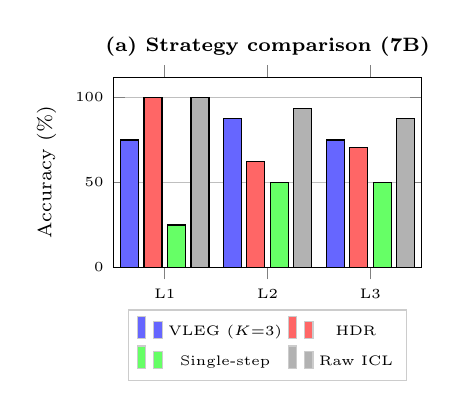
\begin{tikzpicture}
    \begin{axis}[
        ybar, bar width=6.5pt, width=5.5cm, height=4.0cm, enlarge x limits=0.25,
        ylabel={Accuracy (\%)}, symbolic x coords={L1, L2, L3}, xtick=data,
        ymin=0, ymax=112, ymajorgrids=true, tick label style={font=\tiny}, label style={font=\scriptsize},
        title={(a) Strategy comparison (7B)}, title style={font=\scriptsize\bfseries, yshift=-2pt},
        legend style={at={(0.5,-0.22)}, anchor=north, legend columns=2, font=\tiny, draw=gray!40}
    ]
    \addplot[fill=blue!60] coordinates {(L1, 75.0) (L2, 87.5) (L3, 75.0)}; \addlegendentry{VLEG ($K{=}3$)}
    \addplot[fill=red!60] coordinates {(L1, 100.0) (L2, 62.5) (L3, 70.8)}; \addlegendentry{HDR}
    \addplot[fill=green!60] coordinates {(L1, 25.0) (L2, 50.0) (L3, 50.0)}; \addlegendentry{Single-step}
    \addplot[fill=gray!60] coordinates {(L1, 100.0) (L2, 93.8) (L3, 87.5)}; \addlegendentry{Raw ICL}
    \end{axis}
\end{tikzpicture}\hspace{0.20cm}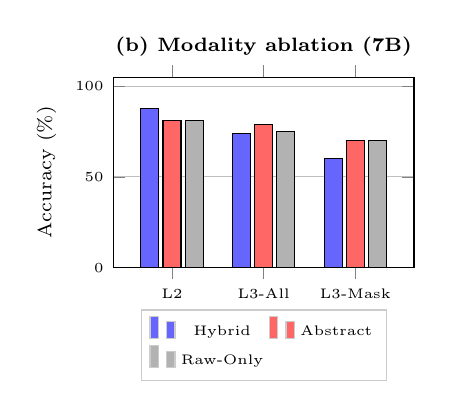
\begin{tikzpicture}
    \begin{axis}[
        ybar=1.5pt, bar width=6.5pt, width=5.4cm, height=4.0cm, enlarge x limits=0.32,
        ylabel={Accuracy (\%)}, symbolic x coords={L2, L3-All, L3-Mask}, xtick=data,
        ymin=0, ymax=105, ymajorgrids=true, tick label style={font=\tiny}, label style={font=\scriptsize},
        title={(b) Modality ablation (7B)}, title style={font=\scriptsize\bfseries, yshift=-2pt},
        legend style={at={(0.5,-0.22)}, anchor=north, legend columns=2, font=\tiny, draw=gray!40}
    ]
    \addplot[fill=blue!60] coordinates {(L2, 87.5) (L3-All, 73.8) (L3-Mask, 60.0)}; \addlegendentry{Hybrid}
    \addplot[fill=red!60] coordinates {(L2, 81.2) (L3-All, 78.8) (L3-Mask, 70.0)}; \addlegendentry{Abstract}
    \addplot[fill=gray!60] coordinates {(L2, 81.2) (L3-All, 75.0) (L3-Mask, 70.0)}; \addlegendentry{Raw-Only}
    \end{axis}
\end{tikzpicture}\hspace{0.20cm}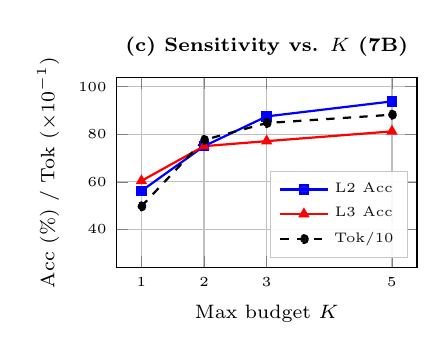
\begin{tikzpicture}
    \begin{axis}[
        width=5.4cm, height=4.0cm, xlabel={Max budget $K$}, ylabel={Acc (\%) / Tok ($\times 10^{-1}$)},
        ymin=24, ymax=104, xtick={1,2,3,5}, grid=major, tick label style={font=\tiny}, label style={font=\scriptsize},
        title={(c) Sensitivity vs. $K$ (7B)}, title style={font=\scriptsize\bfseries, yshift=-2pt},
        legend style={at={(0.97,0.05)}, anchor=south east, legend columns=1, font=\tiny, draw=gray!45, fill=white, fill opacity=0.92}
    ]
    \addplot[color=blue, mark=square*, thick, mark size=1.5pt] coordinates {(1, 56.2) (2, 75.0) (3, 87.5) (5, 93.8)}; \addlegendentry{L2 Acc}
    \addplot[color=red, mark=triangle*, thick, mark size=1.6pt] coordinates {(1, 60.4) (2, 75.0) (3, 77.1) (5, 81.2)}; \addlegendentry{L3 Acc}
    \addplot[color=black, mark=*, thick, dashed, mark size=1.4pt] coordinates {(1, 49.7) (2, 77.6) (3, 84.7) (5, 88.2)}; \addlegendentry{Tok/10}
    \end{axis}
\end{tikzpicture}
\end{adjustbox}
\caption{Summary of the 16-scene symbolic sanity check on Qwen2.5-7B-Instruct: (a) task accuracy across complexity levels ($n=48$ pooled at L3); (b) grounding modality ablation ($n=80$ overall, $n=20$ withheld masked scenes); (c) accuracy and scaled consolidation tokens/episode ($497 \to 882$ tokens) across $K \in \{1,2,3,5\}$.}
\label{fig:symbolic_summary}
\end{figure}

\begin{table}[tbp]
\centering
\caption{Symbolic memory quality and scale comparison across Qwen2.5-7B-Instruct and Llama-3.3-70B-Instruct. ``Spurious Mention'' measures the fraction of label-correct reflections citing non-causal \texttt{texture} or \texttt{size} attributes.}
\label{tab:symbolic_quality}
\footnotesize
\begin{adjustbox}{max width=0.97\textwidth}
\begin{tabular}{@{}llcccc@{}}
\toprule
\textbf{Model Scale} & \textbf{Consolidation Strategy} & \textbf{L3 Admission} & \textbf{Source Label Agreement} & \textbf{Spurious Mention} & \textbf{L3 Test Acc. ($n=48$)} \\
\midrule
\multirow{2}{*}{Qwen2.5-7B} & Unverified Single-Step & Always commit & 41.7\% (5/12) & 80.0\% (4/5) & 50.00\% (24/48) \\
 & VLEG ($K=3$, Stage-A) & 100.0\% (12/12) & \textbf{100.0\% (12/12)} & 83.3\% (10/12) & 75.00\% (36/48) \\
\midrule
\multirow{3}{*}{Llama-3.3-70B} & Raw Retrieval (ICL) / HDR & 100.0\% (12/12) & -- & -- & 89.58\% / 83.33\% \\
 & Multi-Attempt Reflexion & 100.0\% (12/12) & -- & -- & 81.25\% (39/48) \\
 & \textbf{VLEG ($K=3$, Stage-A)} & \textbf{100.0\% (12/12)} & \textbf{100.0\% (12/12)} & \textbf{16.7\% (2/12)} & \textbf{91.67\% (44/48)} \\
\bottomrule
\end{tabular}
\end{adjustbox}
\end{table}

Figure~\ref{fig:symbolic_summary} and Table~\ref{tab:symbolic_quality} establish three foundational properties of Stage-A verification:
\begin{enumerate}[leftmargin=1.8em,topsep=2pt,itemsep=1.5pt]
    \item \textbf{Elimination of Label Inversions and 70B Parity:} Unverified 7B reflections default to \texttt{ANOMALY} ($41.7\%$--$50.0\%$ label correctness), tracking base rates, while global hypothesis induction (HDR) drops from $100.0\%$ at Level~1 to $62.5\%$--$70.8\%$ once rules become background-conditional (Figure~\ref{fig:symbolic_summary}a). Stage-A VLEG restores $100\%$ source-label agreement across both scales and reaches $91.67\%$ ($44/48$) at 70B, matching raw ICL ($89.58\%$, $43/48$) and exceeding HDR ($83.33\%$) and binary-feedback Reflexion ($81.25\%$).
    \item \textbf{Distractor Anchoring in Hybrid Prompts:} At 7B, Hybrid Grounding leads on seen Level-2 scenes ($87.5\%$) but trails single-modality prompts on withheld Level-3 scenes ($60.0\%$ versus $70.0\%$; Figure~\ref{fig:symbolic_summary}b) because 7B reflections mention non-causal \texttt{texture}/\texttt{size} distractors in $83.3\%$--$86.7\%$ of rules. At 70B, spurious mentions drop to $12.5\%$--$16.7\%$ in both verified and unverified proposals alike, lifting Hybrid accuracy to $95.0\%$ overall ($80.0\%$ masked).
    \item \textbf{Coverage Recovery and Concave Cost Growth:} Raising $K$ from $1$ to $3$ lifts 7B Level-3 accuracy by $+11.25$~pp ($63.75\%$ to $75.0\%$) and 70B accuracy by $+26.2 \pm 8.1$~pp by recovering episodes rejected at $j=0$ ($42\%$--$58\%$ admission at $K=1$ versus $83\%$--$100\%$ at $K=3$). Token cost grows concavely ($497 \to 776 \to 847 \to 882$ tokens/episode for $K \in \{1,2,3,5\}$; Figure~\ref{fig:symbolic_summary}c), converging by $K=2$ at 70B. Crucially, single-episode verification guarantees source agreement ($E_j^{\mathrm{src}}=0$) but cannot falsify incidental attributes without cross-episode contrast, motivating Stage-B VLEG-CR on real network flows.
\end{enumerate}

\subsection{Primary Network-Flow Benchmark on Deduplicated UNSW-NB15}
\label{sec:exp6}
\textbf{On deduplicated 19-feature UNSW-NB15 telemetry, coupling Stage-B counterexample refinement with Phase-2 neuro-symbolic execution enables VLEG-CR-NS and VLEG-CR-Bank to significantly outperform raw flow retrieval while cutting online 70B LLM calls by nearly half, and pairing compiled rules with a shallow CART fallback lifts Macro-F1 to 67.05\%--67.57\% without hyperparameter re-tuning at zero online LLM cost.} Applying the 19-feature schema and cross-split deduplication (Section~\ref{sec:features_retrieval}) to UNSW-NB15 compresses the official training split from 175,341 raw rows to 88,699 unique flow fingerprints (purging 79,746 exact duplicates and conflicting rows) and the testing split from 82,332 raw rows to 45,215 disjoint fingerprints (purging 33,161 duplicates and train-overlapping vectors). Five formal seeds (\texttt{20261020}--\texttt{20261024}) each sample a balanced 32-flow support bank (16 benign, 16 malicious; 160 support episodes total) and evaluate the shared 1,000-fingerprint test set (663 benign, 337 malicious), strictly disjoint from the 100-query pilot partition (\texttt{pilot\_20261012}). All LLM methods use Llama-3.3-70B-Instruct (\texttt{Q4\_K\_M}), $K = K_{\mathrm{CR}} = k = 3$, and a 32,768-token context budget.

Why do all 32-flow methods exhibit false positive rates around $36\%$--$42\%$ on this benchmark (Table~\ref{tab:exp6_performance}), whereas prior studies on raw UNSW-NB15 often report $<5\%$ FPR? Two structural data factors govern this operating regime. First, removing the 79,746 repetitive scanning and flood duplicates eliminates trivial majority clusters, raising the FPR floor even for a full-supervision Random Forest trained on all 88,699 unique flows to $22.99\%$ ($31.98\%$ for full-train depth-5 CART and $34.54\%$ for full-train GBDT). Second, sampling balanced 16-benign / 16-malicious few-shot support banks ($50.0\%$ attack prior) against a benign-majority test distribution ($33.7\%$ attack prior) shifts decision boundaries toward attack sensitivity across every leak-free 32-flow learner---including shallow CART (34.96\% FPR), unconstrained CART (36.65\%), GBDT (38.13\%), RF (40.18\%), and raw LLM retrieval ($38.13\%$). Within this shared regime, \textbf{VLEG-CR-Bank achieves a $35.99\% \pm 6.06\%$ FPR}---lowest among all zero-training LLM/neuro-symbolic methods and lower than unconstrained CART (36.65\%), GBDT (38.13\%), and RF (40.18\%), while matching depth-3 CART (34.96\% $\pm$ 8.78\%) with tighter cross-seed stability.

\begin{table}[tbp]
\centering
\caption{Classification performance on the 1,000 shared deduplicated UNSW-NB15 test fingerprints (mean $\pm$ sample SD across five 32-flow seeds). Invalid LLM replies are scored as errors. All few-shot methods and categorical encoders observe strictly the exact same 32 support flows per seed; full-train baselines fit all 88,699 unique training flows.}
\label{tab:exp6_performance}
\footnotesize
\setlength{\tabcolsep}{5.2pt}
\resizebox{0.97\textwidth}{!}{\begin{tabular}{@{}lcccc@{}}
\toprule
\textbf{Method / Supervision Condition} & \textbf{Accuracy (\%)} & \textbf{Macro-F1 (\%)} & \textbf{Attack Recall (\%)} & \textbf{FPR (\%)} \\
\midrule
\multicolumn{5}{@{}l@{}}{\textit{Regime A: Few-Shot LLM \& Neuro-Symbolic Memory (32 flows/seed, $k=3$, 0 gradient updates)}} \\
Raw flow retrieval (shared top-$3$ baseline) & 65.08 $\pm$ 2.93 & 63.92 $\pm$ 2.54 & 71.39 $\pm$ 8.44 & 38.13 $\pm$ 6.85 \\
Raw on Stage-A admitted flows (coverage control) & 64.86 $\pm$ 2.96 & 63.70 $\pm$ 2.68 & 71.16 $\pm$ 8.71 & 38.34 $\pm$ 6.61 \\
Unverified single-step reflection ($j=0$, prompt) & 61.38 $\pm$ 1.08 & 42.66 $\pm$ 1.35 & 6.17 $\pm$ 1.43 & 9.89 $\pm$ 2.03 \\
Global bank summary (single 32-flow prompt) & 50.22 $\pm$ 12.45 & 47.60 $\pm$ 14.13 & \textbf{87.12 $\pm$ 22.27} & 68.54 $\pm$ 24.20 \\
VLEG (Stage-A source-verified, hybrid prompt) & 59.74 $\pm$ 2.03 & 59.68 $\pm$ 2.03 & 77.74 $\pm$ 5.69 & 48.78 $\pm$ 1.67 \\
VLEG-CG (within-seed CE prompt gate fallback) & 64.66 $\pm$ 2.83 & 63.55 $\pm$ 2.49 & 70.27 $\pm$ 8.14 & 37.86 $\pm$ 7.16 \\
VLEG-CR (Stage-B refined, unconditional prompt) & 61.72 $\pm$ 2.40 & 61.45 $\pm$ 2.17 & 78.87 $\pm$ 7.58 & 46.67 $\pm$ 5.07 \\
\textbf{VLEG-CR-NS (Ours, top-$3$ NS + Raw LLM fallback)} & 65.82 $\pm$ 2.49 & 64.88 $\pm$ 2.58 & 74.66 $\pm$ 8.39 & 38.67 $\pm$ 5.06 \\
\textbf{VLEG-CR-Bank (Ours, Pilot $\tau_{\mathrm{sup}}=3$ + Raw LLM)} & \textbf{66.58 $\pm$ 2.79} & \textbf{65.30 $\pm$ 2.74} & 71.63 $\pm$ 9.32 & \textbf{35.99 $\pm$ 6.06} \\
\midrule
\multicolumn{5}{@{}l@{}}{\textit{Regime B: Zero-Online-LLM Neuro-Symbolic + Shallow CART Hybrids (32 flows/seed, 0 LLM calls)}} \\
\textbf{VLEG-CR-Bank (fixed $\tau_{\mathrm{sup}}=3$) + CART ($d=3$) fallback} & 67.92 $\pm$ 2.99 & 67.05 $\pm$ 2.95 & 79.17 $\pm$ 12.32 & 37.80 $\pm$ 6.70 \\
\textbf{VLEG-CR-NS (top-$3$, $\tau_{\mathrm{sup}}=0$) + CART ($d=3$) fallback} & \textbf{68.50 $\pm$ 2.69} & \textbf{67.57 $\pm$ 3.08} & \textbf{79.35 $\pm$ 13.64} & \textbf{37.01 $\pm$ 5.72} \\
\midrule
\multicolumn{5}{@{}l@{}}{\textit{Regime C: Classical Supervised Tabular Baselines (Same 32 flows/seed, strict 32-flow encoder)}} \\
Shallow Decision Tree (CART, depth=3) & 69.88 $\pm$ 1.91 & 68.71 $\pm$ 2.02 & 79.41 $\pm$ 16.27 & \textbf{34.96 $\pm$ 8.78} \\
Decision Tree (CART, unconstrained depth) & \textbf{70.50 $\pm$ 1.91} & \textbf{69.83 $\pm$ 1.62} & 84.57 $\pm$ 9.58 & 36.65 $\pm$ 6.50 \\
Random Forest (200 trees, 32-flow) & 68.92 $\pm$ 1.18 & 68.43 $\pm$ 1.20 & \textbf{86.82 $\pm$ 11.40} & 40.18 $\pm$ 5.90 \\
Gradient Boosting / GBDT (32-flow) & 67.90 $\pm$ 4.15 & 67.12 $\pm$ 4.32 & 79.76 $\pm$ 11.62 & 38.13 $\pm$ 5.86 \\
\midrule
\multicolumn{5}{@{}l@{}}{\textit{Regime D: Full-Supervision Tabular Upper Bounds (All 88,699 unique training flows)}} \\
Shallow Decision Tree (CART, depth=5) & 77.20 $\pm$ 0.00 & 76.81 $\pm$ 0.00 & 95.25 $\pm$ 0.00 & 31.98 $\pm$ 0.00 \\
Random Forest (Full-train upper bound) & \textbf{82.06 $\pm$ 0.36} & \textbf{81.31 $\pm$ 0.36} & 91.99 $\pm$ 0.59 & \textbf{22.99 $\pm$ 0.55} \\
Gradient Boosting / GBDT (Full-train) & 76.50 $\pm$ 0.00 & 76.25 $\pm$ 0.00 & \textbf{98.22 $\pm$ 0.00} & 34.54 $\pm$ 0.00 \\
\bottomrule
\end{tabular}}
\end{table}

\begin{table}[tbp]
\centering
\caption{Phase~1 consolidation and deterministic predicate audit ($\Psi$) across all 160 historical support episodes ($80$ benign, $80$ malicious across five seeds).$^\dagger$}
\label{tab:counterexample_audit}
\footnotesize
\setlength{\tabcolsep}{4.0pt}
\resizebox{0.97\textwidth}{!}{\begin{tabular}{@{}lcccccc@{}}
\toprule
\textbf{Consolidation Stage / Control} & \textbf{Admitted} & \textbf{Benign OK} & \textbf{Malicious OK} & \textbf{Zero $\mathrm{CE}_{\mathrm{seed}}$ (of 160)} & \textbf{Within-Seed CE $>0$} & \textbf{Cross-Seed CE $>0$} \\
\midrule
Stage A, $j{=}0$ (Label-free unverified) & 160 / 160 & 80 / 80 (100\%) & 4 / 80 (5.0\%) & 34 / 160 (21.3\%) & 126 / 160 (78.8\%) & 136 / 160 (85.0\%) \\
Label-given unverified control & 160 / 160 & 80 / 80 (100\%) & 80 / 80 (100\%) & 9 / 160 (5.6\%) & 62 / 71 (87.3\%) & 66 / 71 (93.0\%) \\
Stage A, $j{\le}1$ (1st label-informed rev.) & 95 / 160 & 80 / 80 (100\%) & 15 / 80 (18.8\%) & 41 / 160 (25.6\%) & 53 / 94 (56.4\%) & 67 / 94 (71.3\%) \\
Stage A, $j{\le}2$ (VLEG $K{=}3$ source-only) & 158 / 160 & 80 / 80 (100\%) & 78 / 78 (100\%) & 64 / 160 (40.0\%) & 93 / 157 (59.2\%) & 113 / 157 (72.0\%) \\
\textbf{Stage B (VLEG-CR, $K_{\mathrm{CR}}{=}3$, $v{=}1$)} & \textbf{133 / 158 (84.2\%)} & \textbf{67 / 67 (100\%)} & \textbf{66 / 66 (100\%)} & \textbf{133 / 160 (83.1\%)} & \textbf{0 / 133 (0.0\%)} & \textbf{54 / 133 (40.6\%)} \\
\bottomrule
\end{tabular}}
\par\vspace{2.5pt}
\noindent{\scriptsize $^\dagger$Note: Among the $158/160$ Stage-A VLEG admitted reflections ($j \le 2$), $157$ compile via $\Psi$ and $1$ lacks an explicit \texttt{if-then} clause (hence $93/157$ within-seed CE). Under the Label-given unverified control, $(x_i, y_i)$ is supplied directly at $j=0$ without a verifier: only $71/160$ ($44.4\%$) compile into source-true predicates, $62/71$ ($87.3\%$) match within-seed counterexamples, and $9/160$ ($5.6\%$) reach $\mathrm{CE}_{\mathrm{seed}}=0$. Under strict $v=1$ gating (Algorithm~\ref{alg:vleg_final}), the $2$ Stage-A rejected episodes are excluded from Stage~B, yielding $133$ verified $\mathrm{CE}_{\mathrm{seed}}=0$ rules ($83.1\%$ of all $160$ episodes; $84.2\%$ of the $158$ Stage-A admitted episodes).\par}
\end{table}

\subsubsection{Unverified Collapse, Label-Informed Control, and Iterative Verification Trajectories}
\textbf{Unverified single-step reflection collapses on malicious traffic due to benign-prior bias, and supplying ground-truth labels directly without iterative verification still leaves 94.4\% of episodes either unparseable or falsified by within-seed counterexamples.} At $j=0$ without label access, $\mathcal{G}_\theta$ labels all $80/80$ benign flows as \texttt{BENIGN} but mislabels $76/80$ ($95.0\%$) malicious flows as \texttt{BENIGN}, collapsing test attack recall to 6.17\% (42.66\% Macro-F1; Table~\ref{tab:exp6_performance}). One might ask whether this failure stems merely from withholding $y_i$ at $j=0$. Two empirical controls in Table~\ref{tab:counterexample_audit} refute that hypothesis. First, along VLEG's own verification trajectory, even after the $j=0$ critique explicitly reveals $y_i = \texttt{MALICIOUS}$, a single revision ($j \le 1$) recovers only $11$ of the $76$ rejected malicious episodes ($15/80 = 18.8\%$ malicious admission); a second rejection gate ($j \le 2$) is required to recover $63$ further episodes and reach $158/160$ source-consistent admission (59.68\% Macro-F1). Second, we ran a dedicated \emph{Label-given unverified single-step control} that supplies $(x_i, y_i)$ directly in the $j=0$ prompt across all 160 episodes: although stated labels match $y_i$, only $71/160$ (44.4\%) outputs compile into predicates that hold on $x_i$ itself, $62/71$ (87.3\%) match contrary-label flows in the same seed, and just $9/160$ (5.6\%) achieve valid $\mathrm{CE}_{\mathrm{seed}}=0$ rules. Multi-step verification is therefore essential even when historical labels are known.

\subsubsection{Stage-B Counterexample Refinement and Prompt Anchoring on Non-Firing Rules}
\textbf{Stage-B counterexample refinement more than doubles verified zero-counterexample rule coverage and transfers across unseen seeds, whereas injecting refined rules unconditionally as prompt text triggers false alarms on benign flows even when zero malicious rules fire.} Under Stage-A VLEG, $59.2\%$ ($93/157$) of parseable rules match contrary-label flows within their own 32-flow seed, inflating test FPR to $48.78\%$. Prompt-level gating (VLEG-CG) strips those $93$ rules to curb FPR ($37.86\%$) but leaves usable rules on only $40.0\%$ ($64/160$) of episodes. By feeding concrete contrary-label flows and separating feature bounds back to $\mathcal{G}_\theta$ (illustrated on a real logged episode in Table~\ref{tab:case_study}), Stage-B \textbf{VLEG-CR} raises verified $\mathrm{CE}_{\mathrm{seed}}=0$ coverage across the 160-flow pool from $40.0\%$ ($64/160$) to \textbf{$83.1\%$ ($133/160$, or $84.2\%$ of the $158$ Stage-A admitted episodes: $67/80$ benign and $66/78$ admitted malicious)}. Crucially, within-seed specialization generalizes out-of-sample: unseen cross-seed counterexample incidence ($\mathrm{CE}_{\mathrm{pool}}>0$) drops from $72.0\%$ to \textbf{$40.6\%$ ($54/133$)}, and malicious rules with zero cross-seed counterexamples rise from $35.1\%$ to \textbf{$56.1\%$ ($37/66$)}.

\begin{table}[tbp]
\centering
\caption{Prompt templates and logged four-stage rule trajectory for support episode \texttt{622f0c59...} (Seed \texttt{20261020}, ground truth: \texttt{MALICIOUS}), illustrating how VLEG-CR resolves both label inversion and cross-flow over-generalization.}
\label{tab:case_study}
\footnotesize
\begin{tabularx}{0.98\textwidth}{@{}p{3.0cm}X@{}}
\toprule
\textbf{Pipeline Stage / Role} & \textbf{Exact Prompt Specification or Logged Model / Compiler Output} \\
\midrule
\textbf{Prompt Templates} & \textbf{Generator $\mathcal{G}_\theta$:} \emph{``Analyze a historical network flow. Infer BENIGN or MALICIOUS from the listed flow features and write a concise, testable local heuristic supporting that label. Do not invent payload contents, topology, host roles or fields not supplied... (<700 chars).''} \newline
\textbf{Verifier $\mathcal{V}_\phi$:} \emph{``Check a candidate reflection against ONE historical flow and its known label. Reject if its stated label contradicts the historical label, if it invents a field/value, or if it has no checkable feature condition. Reply with only JSON: \texttt{\{"valid": true/false, "critique": "..."\}}.''} \newline
\textbf{Inference $\mathrm{LLM}_\psi$:} \emph{``Classify the target network flow as BENIGN or MALICIOUS... Reply with exactly one word: BENIGN or MALICIOUS.''} \\
\midrule
\textbf{Source Flow $e_i$ (19 features)} & \texttt{proto="tcp", state="FIN", service="-", dur=0.544, spkts=12, dpkts=6, sbytes=5002, dbytes=268, rate=31.24, sttl=254, dttl=252, sload=67414.4, dload=3292.8, sinpkt=2565.8, dinpkt=5137.5, sjit=276235.0, djit=11277.7, smean=417, dmean=45.} \newline
\textbf{Ground-Truth Historical Label:} \texttt{MALICIOUS} \\
\midrule
\textbf{1. Unverified ($j=0$)} & \texttt{if proto == "tcp" and state == "FIN" and dur < 1 then label = BENIGN} (short-lived normal closure). $\rightarrow$ \textbf{Rejected by $\mathcal{V}_\phi$:} \emph{stated label contradicts historical label.} \\
\textbf{2. Stage-A VLEG ($j=1$)} & \texttt{if proto == "tcp" and state == "FIN" and dur < 1 and sbytes > dbytes then label = MALICIOUS}. $\rightarrow$ \textbf{Passed $\mathcal{V}_\phi$ ($v=1$)}, but \textbf{Rejected by $\Psi$:} matches $\mathrm{CE}_{\mathrm{seed}} = 3$ benign short TCP flows with \texttt{sbytes > dbytes}. \\
\textbf{3. Stage-B Critique $\tilde{c}_i^{(0)}$} & Supplies the 3 falsely matched benign JSON flows + separating bounds (\texttt{dinpkt=5137.5 > max CE}, \texttt{djit=11277.7 > max CE}, \texttt{rate=31.24 > max CE}) + non-memorizing inequality constraint. \\
\textbf{4. Stage-B VLEG-CR ($t=0$)} & \texttt{if dinpkt > 1000 and sbytes > 1000 and rate > 27 and djit > 1000 then label = MALICIOUS} (high inter-packet delay, elevated byte volume, rate, and jitter separate attack from benign closures). $\rightarrow$ \textbf{Accepted:} $\pi(r)(x_i)=1$, $\mathrm{CE}_{\mathrm{seed}} = 0$, and $\mathcal{V}_\phi$ valid ($v=1$). \\
\bottomrule
\end{tabularx}
\end{table}

Unconditionally injecting Stage-B rules into prompts (prompt-only \textbf{VLEG-CR}, showing $\ge 1$ rule on $97.1\%$ of queries) lifts Macro-F1 over Stage-A VLEG from $59.68\%$ to $61.45\%$ and halves invalid replies ($30 \to 15$), yet still suffers a $46.67\%$ FPR. Compiler truth-value auditing pinpoints why: across all \textbf{2,842 benign test evaluations where zero retrieved malicious VLEG-CR rules fired} ($\pi(r_i^{\mathrm{CR}})(x_T)=0$), prompt-only VLEG-CR still produced a \textbf{$39.34\%$ FPR}, versus \textbf{$32.27\%$} for raw flow retrieval on the exact same 2,842 evaluations ($+7.07$~pp). Mere exposure to ``\texttt{then label = MALICIOUS}'' text in non-firing rules biases the quantized 70B model toward false alarms.

\subsubsection{Factorial Ablation and Compute Amortization of Neuro-Symbolic Triage}
\textbf{Deterministic predicate execution eliminates non-firing prompt anchoring and achieves statistically significant Macro-F1 gains over raw retrieval while amortizing offline consolidation cost under 195 queries.} Execution scopes and support thresholds $\tau_{\mathrm{sup}} \in \{0,1,2,3,5\}$ for LLM-fallback bank triage were screened strictly on the disjoint 100-query pilot set (\texttt{pilot\_20261012}). Because that single 32-flow pilot draw contains challenging boundary benign traffic, all baseline learners score in the $52\%$--$55\%$ Macro-F1 range on the pilot set---including Raw flow retrieval ($54.63\%$) and standalone depth-3 CART ($54.53\%$). On the pilot set, VLEG-CR-NS ($\tau_{\mathrm{sup}}=0$) rose to $55.72\%$ and VLEG-CR-Bank peaked at $\tau_{\mathrm{sup}}=3$ with $61.00\%$ Macro-F1. For CART-fallback hybrids, we retain zero-hyperparameter \textbf{VLEG-CR-NS + CART} ($\tau_{\mathrm{sup}}=0$) and fixed-threshold \textbf{VLEG-CR-Bank ($\tau_{\mathrm{sup}}=3$) + CART} without re-tuning on the test set, and report $\tau_{\mathrm{sup}}=5$ in Table~\ref{tab:ns_ablation} solely as a high-support sensitivity point.

\begin{table}[tbp]
\centering
\caption{Factorial ablation of Phase~1 consolidation and Phase~2 execution across the pilot set ($n=100$) and five formal seeds ($5 \times 1,000$ queries). Paired cluster bootstrap $95\%$ CIs compare formal Macro-F1 against Raw flow retrieval ($63.92\%$).}
\label{tab:ns_ablation}
\footnotesize
\setlength{\tabcolsep}{3.6pt}
\noindent\resizebox{0.95\textwidth}{!}{\begin{tabular}{llccccc}
\toprule
\textbf{Phase 1 Rules} & \textbf{Phase 2 Inference Mechanism} & \textbf{Pilot F1} & \textbf{Macro-F1 (\%)} & \textbf{FPR (\%)} & \textbf{Rule Cov.} & \textbf{$\Delta$F1 vs. Raw (95\% CI)\,} \\
\midrule
None (Raw) & LLM prompt over top-$3$ raw flows & 54.63\% & 63.92 $\pm$ 2.54 & 38.13 $\pm$ 6.85 & 0.0\% & Baseline (0.00) \\
None (CART) & Shallow Decision Tree (CART, $d{=}3$) & 54.53\% & 68.71 $\pm$ 2.02 & 34.96 $\pm$ 8.78 & 0.0\% (tree) & $+4.79$ $[+2.95, +6.76]$ \\
Stage-A VLEG & Unconditional hybrid LLM prompt & 48.87\% & 59.68 $\pm$ 2.03 & 48.78 $\pm$ 1.67 & 0.0\% & $-4.24$ $[-5.91, -2.53]$ \\
Stage-A VLEG & Prompt CE gate fallback (VLEG-CG) & 54.63\% & 63.55 $\pm$ 2.49 & 37.86 $\pm$ 7.16 & 0.0\% & $-0.37$ $[-1.18, +0.42]$ \\
Stage-A VLEG & Neuro-symbolic top-$3$ ($\tau_{\mathrm{sup}}{=}0$, no CR) & 54.63\% & 63.99 $\pm$ 2.62 & 40.36 $\pm$ 6.54 & 20.1 $\pm$ 5.4\% & $+0.08$ $[-0.50, +0.63]$ \\
Stage-A VLEG & Neuro-symbolic bank ($\tau_{\mathrm{sup}}{=}3$, no CR) & 54.63\% & 63.52 $\pm$ 2.92 & 41.30 $\pm$ 8.15 & 15.0 $\pm$ 8.7\% & $-0.40$ $[-0.95, +0.19]$ \\
\midrule
Stage-B CR & Unconditional hybrid LLM prompt & 54.78\% & 61.45 $\pm$ 2.17 & 46.67 $\pm$ 5.07 & 0.0\% & $-2.47$ $[-3.90, -0.96]$ \\
Stage-B CR & Active-firing LLM prompt gate (top-$3$) & 55.72\% & 64.11 $\pm$ 2.59 & 40.42 $\pm$ 4.89 & 47.1\% (LLM) & $+0.19$ $[-0.52, +0.95]$ \\
\textbf{Stage-B CR} & \textbf{VLEG-CR-NS (top-$3$ + Raw LLM, $\tau_{\mathrm{sup}}{=}0$)} & 55.72\% & \textbf{64.88 $\pm$ 2.58} & 38.67 $\pm$ 5.06 & \textbf{47.1 $\pm$ 7.2\%} & \textbf{$+0.96$ $[+0.19, +1.71]$} \\
\textbf{Stage-B CR} & \textbf{VLEG-CR-Bank (bank + Raw LLM, $\tau_{\mathrm{sup}}{=}0$)} & 58.50\% & \textbf{65.06 $\pm$ 2.85} & \textbf{35.93 $\pm$ 6.27} & \textbf{68.4 $\pm$ 7.2\%} & $+1.15$ $[-0.30, +2.58]$ \\
\textbf{Stage-B CR} & \textbf{VLEG-CR-Bank (Pilot $\tau_{\mathrm{sup}}{=}3$ + Raw LLM)} & \textbf{61.00\%} & \textbf{65.30 $\pm$ 2.74} & \textbf{35.99 $\pm$ 6.06} & \textbf{49.0 $\pm$ 14.9\%} & \textbf{$+1.38$ $[+0.18, +2.61]$} \\
\midrule
\textbf{Stage-B CR} & \textbf{VLEG-CR-Bank (fixed $\tau_{\mathrm{sup}}{=}3$) + CART ($d{=}3$)} & 51.60\% & \textbf{67.05 $\pm$ 2.95} & 37.80 $\pm$ 6.70 & \textbf{49.0\% (0 LLM)} & \textbf{$+3.13$ $[+1.27, +4.91]$} \\
\textbf{Stage-B CR} & \textbf{VLEG-CR-NS (top-$3$, $\tau_{\mathrm{sup}}{=}0$) + CART ($d{=}3$)} & 52.79\% & \textbf{67.57 $\pm$ 3.08} & 37.01 $\pm$ 5.72 & \textbf{47.1\% (0 LLM)} & \textbf{$+3.65$ $[+1.81, +5.44]$} \\
Stage-B CR & VLEG-CR-Bank ($\tau_{\mathrm{sup}}{=}5$ sensitivity) + CART & 52.08\% & 68.16 $\pm$ 3.47 & 37.10 $\pm$ 7.73 & 33.1\% (0 LLM) & $+4.25$ $[+2.42, +6.20]$ \\
\bottomrule
\end{tabular}}
\end{table}

Table~\ref{tab:ns_ablation} and Figure~\ref{fig:exp6_tradeoff} confirm that both stages are indispensable: applying NS execution to unrefined Stage-A rules covers only $15.0\%$--$20.1\%$ of queries ($+0.08$~pp and $-0.40$~pp vs. Raw), while passing firing CR rules back through the LLM (\texttt{Active-firing LLM prompt gate}, $64.11\%$) loses $0.77$~pp relative to direct symbolic output (\textbf{VLEG-CR-NS}, $64.88\%$, $95\%$ CI $[+0.19, +1.71]$~pp) due to LLM re-interpretation noise. Under Pilot-selected $\tau_{\mathrm{sup}}=3$, \textbf{VLEG-CR-Bank} achieves $65.30\%$ Macro-F1 ($95\%$ CI $[+0.18, +2.61]$~pp) and $35.99\%$ FPR, with $78.54\%$ accuracy on the $49.0\%$ directly rule-resolved subset.

\begin{figure}[tbp]
\centering
\definecolor{cRaw}{HTML}{2B5C8F}
\definecolor{cSingle}{HTML}{A89070}
\definecolor{cVleg}{HTML}{C8523B}
\definecolor{cPromptCR}{HTML}{D9822B}
\definecolor{cNS}{HTML}{2E8B57}
\definecolor{cBank}{HTML}{1B6CA8}
\definecolor{cHyb}{HTML}{0F766E}
\definecolor{cCart}{HTML}{6A4C93}
\begin{adjustbox}{max width=0.98\textwidth}\begin{tikzpicture}
    \begin{axis}[
        ybar, bar width=9.5pt, width=8.4cm, height=5.0cm, enlarge x limits=0.10,
        ylabel={Macro-F1 (\%)}, ymin=0, ymax=84, ytick={0,20,40,60,80},
        symbolic x coords={Single, VLEG, VLEGCR, Raw, CRNS, CRBank, CRNSCART},
        xtick={Single, VLEG, VLEGCR, Raw, CRNS, CRBank, CRNSCART},
        xticklabels={Single, VLEG, VLEG-CR, Raw, CR-NS, CR-Bank, {CR-NS\\+CART}},
        x tick label style={font=\fontsize{5.4}{6.1}\selectfont, align=center}, tick label style={font=\scriptsize}, label style={font=\scriptsize},
        axis lines*=left, clip=false, title={(a) 5-seed Macro-F1 progression},
        title style={at={(0,1.02)}, anchor=south west, font=\footnotesize\bfseries}, bar shift=0pt
    ]
    \addplot[fill=cSingle, draw=black!70, error bars/.cd, y dir=both, y explicit] coordinates {(Single, 42.66) +- (0, 1.35)};
    \addplot[fill=cVleg, draw=black!70, error bars/.cd, y dir=both, y explicit] coordinates {(VLEG, 59.68) +- (0, 2.03)};
    \addplot[fill=cPromptCR, draw=black!70, error bars/.cd, y dir=both, y explicit] coordinates {(VLEGCR, 61.45) +- (0, 2.17)};
    \addplot[fill=cRaw, draw=black!70, error bars/.cd, y dir=both, y explicit] coordinates {(Raw, 63.92) +- (0, 2.54)};
    \addplot[fill=cNS, draw=black!70, error bars/.cd, y dir=both, y explicit] coordinates {(CRNS, 64.88) +- (0, 2.58)};
    \addplot[fill=cBank, draw=black!70, error bars/.cd, y dir=both, y explicit] coordinates {(CRBank, 65.30) +- (0, 2.74)};
    \addplot[fill=cHyb, draw=black!70, error bars/.cd, y dir=both, y explicit] coordinates {(CRNSCART, 67.57) +- (0, 3.08)};

    \node[above, font=\tiny] at (axis cs:Single,44.8) {42.7};
    \node[above, font=\tiny] at (axis cs:VLEG,62.3) {59.7};
    \node[above, font=\tiny] at (axis cs:VLEGCR,64.2) {61.5};
    \node[above, font=\tiny] at (axis cs:Raw,67.0) {63.9};
    \node[above, font=\tiny\bfseries] at (axis cs:CRNS,68.0) {64.9};
    \node[above, font=\tiny\bfseries] at (axis cs:CRBank,68.6) {65.3};
    \node[above, font=\tiny\bfseries] at (axis cs:CRNSCART,71.3) {67.6};
    \end{axis}
\end{tikzpicture}\hspace{0.26cm}\begin{tikzpicture}
    \begin{axis}[
        width=7.6cm, height=5.0cm, xlabel={False positive rate (\%)}, ylabel={Attack recall (\%)},
        xmin=5, xmax=54, ymin=0, ymax=102, xtick={10,20,30,40,50}, ytick={0,20,40,60,80,100},
        tick label style={font=\scriptsize}, label style={font=\scriptsize},
        axis lines*=left, grid=major, title={(b) Recall vs. FPR operating points},
        title style={at={(0,1.02)}, anchor=south west, font=\footnotesize\bfseries},
        legend columns=2,
        legend style={
            at={(0.98,0.04)}, anchor=south east,
            font=\fontsize{5.5}{6.6}\selectfont,
            inner sep=1.8pt, column sep=3pt,
            draw=gray!50, fill=white, fill opacity=0.95,
            cells={anchor=west}
        }
    ]
    \addplot[only marks, mark=diamond*, mark size=3.0pt, color=cSingle] coordinates {(9.89, 6.17)}; \addlegendentry{Single-step}
    \addplot[only marks, mark=triangle*, mark size=3.2pt, color=cVleg] coordinates {(48.78, 77.74)}; \addlegendentry{VLEG (prompt)}
    \addplot[only marks, mark=pentagon*, mark size=3.2pt, color=cPromptCR] coordinates {(46.67, 78.87)}; \addlegendentry{VLEG-CR (prompt)}
    \addplot[only marks, mark=*, mark size=2.9pt, color=cRaw] coordinates {(38.13, 71.39)}; \addlegendentry{Raw retrieval}
    \addplot[only marks, mark=square*, mark size=2.9pt, color=cNS] coordinates {(38.67, 74.66)}; \addlegendentry{VLEG-CR-NS}
    \addplot[only marks, mark=triangle*, mark options={rotate=180}, mark size=3.5pt, color=cBank] coordinates {(35.99, 71.63)}; \addlegendentry{VLEG-CR-Bank}
    \addplot[only marks, mark=oplus*, mark size=3.1pt, thick, color=cHyb] coordinates {(37.01, 79.35)}; \addlegendentry{CR-NS+CART}
    \addplot[only marks, mark=otimes*, mark size=3.1pt, thick, color=cCart] coordinates {(34.96, 79.41)}; \addlegendentry{CART (depth=3)}
    \node[font=\fontsize{5.3}{6.2}\selectfont, text=cVleg!85!black, align=center, anchor=south] at (axis cs:46.8, 85.5) {Prompt-anchored\\[-0.5pt]FPR shift};
    \end{axis}
\end{tikzpicture}\end{adjustbox}
\caption{UNSW-NB15 five-seed performance summary: (a) Macro-F1 ($\pm$ SD) across LLM, neuro-symbolic, and zero-hyperparameter CR-NS+CART variants; (b) attack recall vs. FPR operating trade-offs with all eight baselines clearly separated above the legend.}
\label{fig:exp6_tradeoff}
\end{figure}

\begin{table}[tbp]
\centering
\caption{Offline memory consolidation and online per-query inference cost audit (5-seed means, 32 support flows and 1,000 test queries per seed). Compiled Python predicates execute within $0.1$~ms on CPU.}
\label{tab:exp6_cost}
\footnotesize
\setlength{\tabcolsep}{4.4pt}
\resizebox{0.97\textwidth}{!}{\begin{tabular}{@{}lrrrrrr@{}}
\toprule
\textbf{Condition / Method} & \textbf{Cons. Calls} & \textbf{Cons. Tokens} & \textbf{Cons. (s)} & \textbf{LLM Calls / 1k} & \textbf{Query Tok. / 1k} & \textbf{Mean Lat. (s)} \\
\midrule
Raw flow retrieval & 0.0 & 0 & 0.0 & 1,000.0 & 904,200 & 2.12 \\
Unverified single-step ($j=0$) & 32.0 & 9,405 & 126.5 & 1,000.0 & 982,500 & 2.23 \\
Stage-A VLEG ($K=3$, prompt) & 120.4 & 40,094 & 419.4 & 1,000.0 & 976,800 & 1.74 \\
Stage-B VLEG-CR (prompt-only) & 168.4 & 82,324 & 984.1 & 1,000.0 & 990,800 & 1.81 \\
\textbf{VLEG-CR-NS (top-$3$ + Raw LLM)} & 168.4 & 82,324 & 984.1 & \textbf{529.0 ($-47.1\%$)} & \textbf{478,300} & \textbf{1.12} \\
\textbf{VLEG-CR-Bank ($\tau_{\mathrm{sup}}{=}3$ + Raw LLM)} & 168.4 & 82,324 & 984.1 & \textbf{510.0 ($-49.0\%$)} & \textbf{461,100} & \textbf{1.08} \\
\textbf{VLEG-CR-NS + CART ($d{=}3$, top-$3$)} & 168.4 & 82,324 & 984.1 & \textbf{0.0 ($-100.0\%$)} & \textbf{0} & \textbf{0.08} \\
\textbf{VLEG-CR-Bank ($\tau_{\mathrm{sup}}{=}3$) + CART ($d{=}3$)} & 168.4 & 82,324 & 984.1 & \textbf{0.0 ($-100.0\%$)} & \textbf{0} & \textbf{$< 0.0002$} \\
\bottomrule
\end{tabular}}
\end{table}

Table~\ref{tab:exp6_cost} quantifies end-to-end token and latency budgets. Stage-B refinement adds 48.0 calls and 42,230 tokens per 32-flow seed (82,324 consolidation tokens total). Because VLEG-CR-NS and VLEG-CR-Bank resolve $47.1\%$--$49.0\%$ of test flows within $0.1$~ms on CPU without calling the 70B LLM, they save 425,900--443,100 query tokens per 1,000 flows and halve mean query latency ($2.12$~s to $1.08$--$1.12$~s), amortizing the entire consolidation budget in 186 queries for VLEG-CR-Bank and 194 queries for VLEG-CR-NS (under 195 queries for both).

\subsection{Complementary Positioning Against Shallow Decision Trees and Zero-LLM Hybrids}
\label{sec:exp7}
\textbf{While standalone shallow CART trees achieve higher recall via global impurity optimization, VLEG-CR rules deliver higher precision on covered traffic, tighter false-alarm stability, relational cross-feature auditability, and zero-LLM hybridization.} Comparing Regimes A, B, and C in Table~\ref{tab:exp6_performance} clarifies why neuro-symbolic memory and decision trees are complementary rather than mutually exclusive:
\begin{enumerate}[leftmargin=1.8em,topsep=2pt,itemsep=2pt]
    \item \textbf{Diagnosing the Recall Gap and Eliminating Online Neural Cost:} Under identical 32-flow support encoding, standalone depth-3 CART (68.71\% Macro-F1, 79.41\% recall, 34.96\% FPR) outperforms pure LLM-fallback VLEG-CR-Bank ($65.30\%$ Macro-F1) by $+3.41$~pp. Subset decomposition reveals that on the $49.0\%$ of queries where VLEG-CR-Bank ($\tau_{\mathrm{sup}}=3$) rules fire, deterministic rule accuracy is \textbf{$78.54\%$} ($77.29\%$ for VLEG-CR-NS on $47.1\%$ of queries), substantially higher than standalone CART's 69.88\%; the Macro-F1 gap arises solely on the uncovered boundary flows where zero-shot Raw LLM fallback under-recalls subtle attacks. Replacing the 70B LLM fallback with the exact same 32-flow depth-3 CART tree without re-tuning $\tau_{\mathrm{sup}}$ eliminates $100\%$ of online LLM calls and raises Macro-F1 to \textbf{$67.05\%$} (\textbf{VLEG-CR-Bank + CART}, within $0.2$~ms pure CPU and zero embedding calls via lazy retrieval in Algorithm~\ref{alg:vleg_final}) and \textbf{$67.57\%$} (\textbf{VLEG-CR-NS + CART}, $\tau_{\mathrm{sup}}=0$), matching or surpassing 32-flow GBDT (67.12\% Macro-F1, 38.13\% FPR) in Macro-F1 while achieving lower false positive rates ($37.80\%$ and $37.01\%$) and tighter cross-seed FPR stability ($\pm 5.72\%$ for VLEG-CR-NS + CART versus $\pm 8.78\%$ for standalone depth-3 CART). Tightening support to $\tau_{\mathrm{sup}}=5$ in a sensitivity check reaches $68.16\%$ Macro-F1 while preserving verified rules on $33.1\%$ of queries (Table~\ref{tab:ns_ablation}).
    \item \textbf{Cross-Feature Relational Expressiveness and Modular Rule Governance:} Axis-aligned CART trees test single features against scalar thresholds (e.g., \texttt{sttl <= 46.50} $\to$ \texttt{BENIGN}; \texttt{dinpkt <= 67.08} $\to$ \texttt{MALICIOUS}), which cannot express directional ratios or protocol semantics and must be globally regrown when false-alarm signatures change \cite{jacobs2022ai}. VLEG-CR rules directly encode cross-feature relations such as \texttt{sbytes > dbytes} paired with human-verifiable protocol explanations, allowing SOC analysts to inspect, edit, or revoke individual episodic rules modularly.
\end{enumerate}

\subsection{Limitations}
\label{sec:limitations}
Three limitations bound this study. First, our symbolic sanity check isolates Stage-A verification mechanics on a small synthetic oracle, and shifting from Qwen2.5-7B to Llama-3.3-70B changes model family alongside scale. Second, our primary network evaluation focuses on binary anomaly triage over 19 deduplicated UNSW-NB15 flow features using a single quantized 70B generator; extending VLEG-CR-NS to multi-class attack categorization and additional traffic benchmarks such as CICIDS2017 \cite{sharafaldin2018cicids} or NF-UNSW-NB15-v2 is an important next step. Third, although routing uncovered flows to a shallow CART fallback closes most of the recall gap at zero online LLM cost, joint optimization of relational LLM predicates and tree split thresholds remains open for future work.

\section{Conclusions}
We presented Verified Localized Episodic Grounding (VLEG), Counterexample-Refined consolidation (VLEG-CR), and Neuro-Symbolic rule triage (VLEG-CR-NS and VLEG-CR-Bank) for auditable few-shot network traffic analysis. Our experiments across synthetic scenes and deduplicated UNSW-NB15 network telemetry demonstrate four key findings:
\begin{enumerate}[leftmargin=1.8em,topsep=2pt,itemsep=2pt]
    \item \textbf{Necessity of Multi-Step Source Verification:} Unverified local reflections suffer severe malicious-to-benign label collapse on network telemetry, and even providing ground-truth labels in an unverified single-step prompt leaves over $94\%$ of episodes either unparseable or falsified by within-bank counterexamples. Iterative verification restores full source-label fidelity across admitted episodes.
    \item \textbf{Transferable Specificity via Counterexample-Guided Refinement:} Feeding within-seed counterexamples and separating feature bounds back to the generator more than doubles zero-counterexample rule coverage ($40.0\%$ to $83.1\%$ of all support flows) and cuts unseen cross-seed false matches by over thirty percentage points without memorizing continuous float literals.
    \item \textbf{Elimination of Non-Firing Prompt Anchoring via Neuro-Symbolic Triage:} Displaying non-firing malicious rules in LLM prompts inflates false positives on benign traffic through textual anchoring. Executing compiled zero-counterexample predicates deterministically prior to raw-retrieval fallback delivers statistically significant Macro-F1 gains of up to $+1.38$ percentage points over raw retrieval, reduces false alarms below raw retrieval and 32-flow tree ensembles, and cuts online 70B LLM calls by nearly half.
    \item \textbf{Zero-Online-LLM Synergy with Shallow Decision Trees:} Combining high-precision VLEG-CR relational rules on covered flows with a shallow 32-flow CART fallback on uncovered boundary flows eliminates $100\%$ of online LLM inference cost (and $100\%$ of online embedding cost in Bank scope) while matching or surpassing 32-flow GBDT in Macro-F1 with consistently lower false-alarm rates and retaining human-auditable protocol explanations for SOC triage.
\end{enumerate}

\vspace{0.7em}
{\fontsize{10}{12.5}\selectfont
\noindent\textbf{Acknowledgement:} The authors thank the anonymous reviewers and editors for their constructive comments.\par\vspace{0.25em}
\noindent\textbf{Funding Statement:} This research was funded by the Science and Technology Projects of Ngari Prefecture, Xizang Autonomous Region, China, under Grant No. QYXTZX-AL2026-01.\par\vspace{0.25em}
\noindent\textbf{Author Contributions:} The authors confirm contribution to the paper as follows: study conception and design: Ye Tang, Ruikai Han, Ruzhen Chen; data collection and curation: Ye Tang, Yi Hu; methodology and software: Ye Tang, Ruikai Han; analysis and interpretation of results: Ye Tang, Ruikai Han, Yi Hu; draft manuscript preparation: Ye Tang, Ruikai Han; manuscript review, editing, and supervision: Yi Hu, Ruzhen Chen. All authors reviewed the results and approved the final version of the manuscript.\par\vspace{0.25em}
\noindent\textbf{Availability of Data and Materials:} The public network traffic benchmark evaluated in this study utilizes the publicly available UNSW-NB15 dataset \cite{moustafa2015unsw}. All symbolic benchmark definitions, deterministic compiler scripts, counterexample-refinement checkpoints, and evaluation logs are openly archived for full reproducibility at \linebreak[3]\href{https://github.com/creativitysurvey/VLEG}{\texttt{https://github.com/creativitysurvey/VLEG}}.\par\vspace{0.25em}
\noindent\textbf{Ethics Approval:} Not applicable.\par\vspace{0.25em}
\noindent\textbf{Conflicts of Interest:} The authors declare no conflicts of interest to report regarding the present study.\par
}


\begin{thebibliography}{99}
\fontsize{9.5}{11.5}\selectfont
\setlength{\itemsep}{0.5pt}\setlength{\parsep}{0pt}

\bibitem{brown2020language}
T. B. Brown, B. Mann, N. Ryder, M. Subbiah, J. Kaplan, P. Dhariwal, et al., ``Language models are few-shot learners,'' \emph{Adv. Neural Inf. Process. Syst.}, vol. 33, pp. 1877--1901, 2020.

\bibitem{lewis2020retrieval}
P. Lewis, E. Perez, A. Piktus, F. Petroni, V. Karpukhin, N. Goyal, et al., ``Retrieval-augmented generation for knowledge-intensive NLP tasks,'' \emph{Adv. Neural Inf. Process. Syst.}, vol. 33, pp. 9459--9474, 2020.

\bibitem{lin2022etbert}
X. Lin, G. Xiong, G. Gou, Z. Li, J. Shi, and J. Yu, ``ET-BERT: A contextualized datagram representation with pre-training transformers for encrypted traffic classification,'' in \emph{Proc. ACM Web Conf. (WWW)}, Apr. 2022, pp. 633--642.

\bibitem{sharafaldin2018cicids}
I. Sharafaldin, A. H. Lashkari, and A. A. Ghorbani, ``Toward generating a new intrusion detection dataset and intrusion traffic characterization,'' in \emph{Proc. Int. Conf. Inf. Syst. Secur. Privacy (ICISSP)}, Jan. 2018, pp. 108--116.

\bibitem{papamartzivanos2018dendron}
D. Papamartzivanos, F. G. M\'armol, and G. Kambourakis, ``Dendron: Genetic trees driven rule induction for network intrusion detection systems,'' \emph{Future Gener. Comput. Syst.}, vol. 79, pp. 558--574, 2018.

\bibitem{jacobs2022ai}
A. S. Jacobs, R. Beltiukov, W. Willinger, R. A. Ferreira, A. Gupta, and L. Z. Granville, ``AI/ML for network security: The emperor has no clothes,'' in \emph{Proc. ACM SIGSAC Conf. Comput. Commun. Secur. (CCS)}, Nov. 2022, pp. 1537--1551.

\bibitem{wei2023xaiids}
S. Arisdakessian, O. A. Wahab, A. Mourad, H. Otrok, and M. Guizani, ``A survey on explainable AI for cybersecurity: Architecture, models, and future directions,'' \emph{IEEE Commun. Surveys Tuts.}, vol. 25, no. 4, pp. 2742--2781, 2023.

\bibitem{charmet2022explainable}
F. Charmet, H. C. Tanuwidjaja, S. Ayoubi, P. F. Gimenez, Y. Han, H. Jmila, et al., ``Explainable artificial intelligence for cybersecurity: A literature survey,'' \emph{Ann. Telecommun.}, vol. 77, pp. 787--812, 2022.

\bibitem{houssel2024explainable}
P. R. B. Houssel, P. Singh, S. Layeghy, and M. Portmann, ``Towards explainable network intrusion detection using large language models,'' in \emph{Proc. IEEE Conf. Local Comput. Netw. Workshops (LCN)}, Oct. 2024, pp. 1--6.

\bibitem{islam2026maids}
M. S. Islam, L. G. Jaimes, and A. S. Dina, ``MA-IDS: Multi-agent RAG framework for IoT network intrusion detection with an experience library,'' \emph{arXiv preprint arXiv:2604.05458}, 2026.

\bibitem{guastalla2024llmdos}
M. Guastalla, Y. Li, A. Hekmati, and B. Krishnamachari, ``Application of large language models to DDoS attack detection,'' in \emph{Proc. Int. Conf. Secur. Privacy Cyber-Phys. Syst. Smart Vehicles}, 2024, pp. 83--99.

\bibitem{an2025why}
C. An, J. Zhang, M. Zhong, L. Li, S. Gong, Y. Luo, et al., ``Why does the effective context length of LLMs fall short?'' in \emph{Proc. Int. Conf. Learn. Represent. (ICLR)}, Apr. 2025.

\bibitem{liu2024lost}
N. F. Liu, K. Lin, J. Hewitt, A. Paranjape, M. Bevilacqua, F. Petroni, and P. Liang, ``Lost in the middle: How language models use long contexts,'' \emph{Trans. Assoc. Comput. Linguist.}, vol. 12, pp. 157--173, 2024.

\bibitem{packer2023memgpt}
C. Packer, S. Wooders, K. Lin, V. Fang, S. G. Patil, I. Stoica, and J. E. Gonzalez, ``MemGPT: Towards LLMs as operating systems,'' \emph{arXiv preprint arXiv:2310.08560}, 2023.

\bibitem{wang2023longmem}
W. Wang, L. Dong, H. Cheng, X. Liu, X. Yan, J. Gao, and F. Wei, ``Augmenting language models with long-term memory,'' \emph{Adv. Neural Inf. Process. Syst.}, vol. 36, pp. 74530--74543, 2023.

\bibitem{wang2024memoryllm}
Y. Wang, Y. Gao, X. Chen, H. Jiang, S. Li, J. Yang, et al., ``MEMORYLLM: Towards self-updatable large language models,'' in \emph{Proc. 41st Int. Conf. Mach. Learn. (ICML)}, vol. 235, Jul. 2024, pp. 50453--50466.

\bibitem{gutierrez2024hipporag}
B. Jimenez Gutierrez, Y. Shu, Y. Gu, M. Yasunaga, and Y. Su, ``HippoRAG: Neurobiologically inspired long-term memory for large language models,'' \emph{Adv. Neural Inf. Process. Syst.}, vol. 37, pp. 59532--59569, 2024.

\bibitem{maharana2024evaluating}
A. Maharana, D. H. Lee, S. Tulyakov, M. Bansal, F. Barbieri, and Y. Fang, ``Evaluating very long-term conversational memory of LLM agents,'' in \emph{Proc. 62nd Annu. Meeting Assoc. Comput. Linguist. (ACL)}, Aug. 2024, pp. 13851--13870.

\bibitem{wu2025from}
Y. Wu, S. Liang, C. Zhang, Y. Wang, Y. Zhang, H. Guo, et al., ``From human memory to AI memory: A survey on memory mechanisms in the era of LLMs,'' \emph{arXiv preprint arXiv:2504.15965}, 2025.

\bibitem{zhang2025survey}
Z. Zhang, X. Bo, C. Ma, R. Li, X. Chen, Q. Dai, et al., ``A survey on the memory mechanism of large language model-based agents,'' \emph{ACM Trans. Inf. Syst.}, vol. 43, no. 6, pp. 1--47, 2025.

\bibitem{shinn2023reflexion}
N. Shinn, F. Cassano, A. Gopinath, K. R. Narasimhan, and S. Yao, ``Reflexion: Language agents with verbal reinforcement learning,'' \emph{Adv. Neural Inf. Process. Syst.}, vol. 36, pp. 8634--8652, 2023.

\bibitem{wang2024voyager}
G. Wang, Y. Xie, Y. Jiang, A. Mandlekar, C. Xiao, Y. Zhu, et al., ``Voyager: An open-ended embodied agent with large language models,'' \emph{Trans. Mach. Learn. Res.}, pp. 1--32, 2024.

\bibitem{agarwal2026hypothesis}
A. K. Agarwal and M. Yamada, ``Hypothesis-driven reasoning for large language models,'' in \emph{Proc. 40th AAAI Conf. Artif. Intell. (AAAI)}, Feb. 2026, pp. 1686--1693.

\bibitem{he2024idea}
K. He, M. Zhang, S. Yan, P. Wu, and Z. Chen, ``IDEA: Enhancing the rule learning ability of large language model agent through induction, deduction, and abduction,'' in \emph{Proc. Annu. Meeting Assoc. Comput. Linguist. (ACL)}, Aug. 2024.

\bibitem{moustafa2015unsw}
N. Moustafa and J. Slay, ``UNSW-NB15: A comprehensive data set for network intrusion detection systems (UNSW-NB15 network data set),'' in \emph{Proc. Mil. Commun. Inf. Syst. Conf. (MilCIS)}, Nov. 2015, pp. 1--6.

\bibitem{zhang2022active}
Y. Zhang, S. Feng, and C. Tan, ``Active example selection for in-context learning,'' in \emph{Proc. Conf. Empirical Methods Natural Lang. Process. (EMNLP)}, Dec. 2022, pp. 9134--9148.

\bibitem{purohit2025sample}
K. Purohit, V. V, S. Bhattacharya, and A. Anand, ``Sample efficient demonstration selection for in-context learning,'' in \emph{Proc. 42nd Int. Conf. Mach. Learn. (ICML)}, Jul. 2025.

\bibitem{zhong2024memorybank}
W. Zhong, L. Guo, Q. Gao, H. Ye, and Y. Wang, ``MemoryBank: Enhancing large language models with long-term memory,'' \emph{Proc. AAAI Conf. Artif. Intell.}, vol. 38, pp. 19724--19731, 2024.

\bibitem{park2023generative}
J. S. Park, J. C. O'Brien, C. J. Cai, M. R. Morris, P. Liang, and M. S. Bernstein, ``Generative agents: Interactive simulacra of human behavior,'' in \emph{Proc. 36th Annu. ACM Symp. User Interface Softw. Technol. (UIST)}, Oct. 2023, pp. 1--22.

\bibitem{xu2025amem}
W. Xu, Z. Liang, K. Mei, H. Gao, J. Tan, and Y. Zhang, ``A-MEM: Agentic memory for LLM agents,'' in \emph{Adv. Neural Inf. Process. Syst. (NeurIPS)}, Dec. 2025.

\bibitem{kim2024towards}
S. H. Kim, K. T. Ong, T. Kwon, N. Kim, K. Ka, S. Bae, et al., ``Towards lifelong dialogue agents via timeline-based memory management,'' in \emph{Proc. Conf. North Amer. Chapter Assoc. Comput. Linguist. (NAACL)}, Jun. 2024.

\bibitem{madaan2023selfrefine}
A. Madaan, N. Tandon, P. Gupta, S. Hallinan, L. Gao, S. Wiegreffe, et al., ``Self-Refine: Iterative refinement with self-feedback,'' \emph{Adv. Neural Inf. Process. Syst.}, vol. 36, pp. 46534--46594, 2023.

\bibitem{manakul2023selfcheckgpt}
P. Manakul, A. Liusie, and M. Gales, ``SelfCheckGPT: Zero-resource black-box hallucination detection for generative large language models,'' in \emph{Proc. Conf. Empirical Methods Natural Lang. Process. (EMNLP)}, Dec. 2023, pp. 9004--9017.

\bibitem{dhuliawala2024chain}
S. Dhuliawala, M. Komeili, J. Xu, R. Raileanu, X. Li, A. Celikyilmaz, and J. Weston, ``Chain-of-verification reduces hallucination in large language models,'' in \emph{Findings Assoc. Comput. Linguist. (ACL)}, Aug. 2024, pp. 3563--3578.

\bibitem{gou2024critic}
Z. Gou, Z. Shao, Y. Gong, Y. Shen, Y. Yang, N. Duan, and W. Chen, ``CRITIC: Large language models can self-correct with tool-interactive critiquing,'' in \emph{Proc. Int. Conf. Learn. Represent. (ICLR)}, May 2024.

\bibitem{kim2022playgrounds}
S. Kim, P. Phunyaphibarn, D. Ahn, and S. Kim, ``Playgrounds for abstraction and reasoning,'' in \emph{Proc. NeurIPS Workshop Neuro Causal Symbolic AI}, Dec. 2022.

\bibitem{qiu2024phenomenal}
L. Qiu, L. Jiang, X. Lu, M. Sclar, V. Pyatkin, C. Bhagavatula, et al., ``Phenomenal yet puzzling: Testing inductive reasoning capabilities of language models with hypothesis refinement,'' in \emph{Proc. Int. Conf. Learn. Represent. (ICLR)}, May 2024, pp. 1452--1481.

\bibitem{lee2025generating}
K. I. Lee, H. Koh, D. Lee, S. Yoon, M. Kim, and K. Jung, ``Generating diverse hypotheses for inductive reasoning,'' in \emph{Proc. Int. Conf. Learn. Represent. (ICLR)}, Apr. 2025.

\bibitem{zhou2024hypothesis}
Y. Zhou, H. Liu, T. Srivastava, H. Mei, and C. Tan, ``Hypothesis generation with large language models,'' in \emph{Proc. EMNLP Workshop NLP for Science}, Nov. 2024.

\bibitem{kim2023machine}
T. Kim, M. Cochez, V. Fran\c{c}ois-Lavet, M. Neerincx, and P. Vossen, ``A machine with short-term, episodic, and semantic memory systems,'' \emph{Proc. AAAI Conf. Artif. Intell.}, vol. 37, pp. 48--56, 2023.

\bibitem{li2024memory}
J. Li and J. Li, ``Memory, consciousness and large language model,'' \emph{arXiv preprint arXiv:2401.02509}, 2024.

\bibitem{wang2025mirix}
Y. Wang and X. Chen, ``MIRIX: Multi-agent memory system for LLM-based agents,'' \emph{arXiv preprint arXiv:2507.07957}, 2025.

\bibitem{mirsky2018kitsune}
Y. Mirsky, T. Doitshman, Y. Elovici, and A. Shabtai, ``Kitsune: An ensemble of autoencoders for online network intrusion detection,'' in \emph{Proc. Netw. Distrib. Syst. Secur. Symp. (NDSS)}, Feb. 2018, pp. 1--15.

\bibitem{arp2022dos}
D. Arp, E. Quiring, F. Pendlebury, A. Warnecke, F. Pierazzi, C. Wressnegger, et al., ``Dos and don'ts of machine learning in computer security,'' in \emph{Proc. 31st USENIX Secur. Symp.}, Aug. 2022, pp. 3971--3988.

\bibitem{alissa2022botnet}
K. Alissa, T. Alyas, K. Zafar, Q. Abbas, N. Tabassum, and S. Sakib, ``Botnet detection in IoT using machine learning,'' \emph{Comput. Mater. Continua}, vol. 72, no. 3, pp. 5027--5042, 2022.

\end{thebibliography}

\end{document}
